\documentclass[12pt,a4paper,notitlepage]{article}
\usepackage[framed,numbered,autolinebreaks]{mcode}
\usepackage[margin=1in]{geometry}
\usepackage{amsmath}
\usepackage{amsfonts}
\usepackage{amssymb}
\usepackage{graphicx}
\usepackage{color}
\usepackage{float}
\usepackage[toc,page]{appendix}
\usepackage{parskip}
\usepackage{sectsty}
\usepackage{gensymb}
\usepackage{titlesec}
\usepackage{listings}
\usepackage{titling}
\usepackage{multirow}
\setlength{\droptitle}{-1cm}
\usepackage{enumitem}
\setlist[enumerate]{topsep=0pt,itemsep=-3.5ex,partopsep=1ex,parsep=1ex}
\renewcommand{\rmdefault}{ptm}
\sectionfont{\fontsize{12}{0}\selectfont}
\subsectionfont{\fontsize{12}{0}\selectfont}

% Header and Footer
\setlength{\headheight}{15pt} 
\usepackage{fancyhdr}
\fancypagestyle{plain}{
 \fancyhf{}
 \fancyhead[L]{AA 279C: Spacecraft Attitude Determination and Control}
 \fancyhead[R]{Stanford University}
 \fancyfoot[C]{\thepage}
}

% Table of contents
\setcounter{tocdepth}{5}

\begin{document}
\title{\Huge \textbf{SATELLITE DYNAMICS AND ATTITUDE CONTROL}}
\author{Anna Hylbert and Kristopher Riordan}
\date{10 April 2024}

\begin{minipage}[h]{\textwidth}
	\vspace{4 cm}
	\advance\leftskip-1in
    \maketitle
\end{minipage}

\begin{figure}[H]
\centering
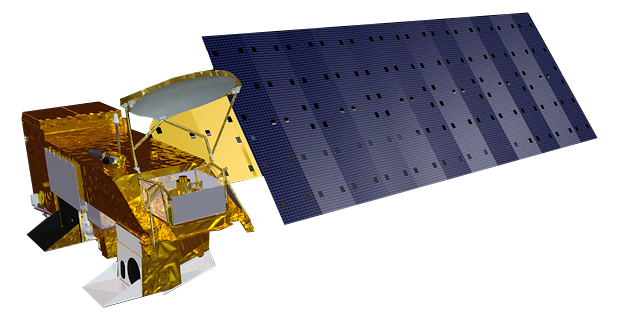
\includegraphics[width = 15cm]{Images/Aqua_spacecraft_model.png}
\end{figure}

\pagebreak

\section*{\Large REVISION HISTORY}

\begin{table}[h!]
\begin{center}
\begin{tabular} [0.9 \textwidth]{cl}
\hline \hline
\multicolumn{1}{c}{VERSION} & \multicolumn{1}{l}{REVISION NOTES} \\
\hline
PS1 & - Created document \\
    & - Added PS1 material \\
\hline
PS2 & - Cleaned up previous references and plots in PS1 material \\
    & - Added euler propagation plots and analysis \\
    & - Added orbit propagation plots and analysis \\
    & - formatted references and added necessary citations \\
\hline
PS3 & - Revised PS2 plots in order to better show numerical integration results\\
    & - \\
\hline \hline
\end{tabular}
	\caption{Summary of project revisions.}
\end{center}
\end{table}
 
\newpage
\section*{\Large TABLE OF CONTENTS}
\makeatletter
\@starttoc{toc}
\makeatother
\newpage
%%%%%%%%%%%%%%%%%%%%%%%%%%%%%%%%%%%%%%%%%%%%%%%%%%%%%%%%%%%%%%%%%%%%%%%%%%%%%%%%%%%%%%%%%%%%%%%%%%%%%%%%%%%%%%%%%%%%%%%%%%%%%%%%%%%%%%%%%%%%%%%%%%%%%%%%%%%%%%%%%%%%%%%%%%%%%%%%%%%%%%%%%%%%%%%%%%%%%%%%%%%%%%%%%%%%%%%%%%%

\section{\Large INTRODUCTION}

\section{\Large PROBLEM SET 1}
\subsection{PROBLEM 1}

\subsubsection{Select the characteristics of your mission.} \label{sec:char}

For this mission, we have decided to create an attitude determination and control system (ADCS) for a Low Earth Orbit (LEO) satellite that is Earth pointing. We are currently planning to use Euler Angles for our attitude state representation as we do not currently believe that the attitude adjustments needed for this mission will be large enough to lead to gimbal lock, the most typical problem that is faced when working with Euler angles. For the satellite's sensors, we are planning to use a magnetometer due to its reliability and a star tracker due to its high precision. The actuators that we are planning to use are reaction wheels and magnetorquers in order to have both large adjustment and fine tuning attitude maneuver capabilities.

\subsubsection{Conduct survey of satellites which have characteristics similar to selected project.}

Outside of communications satellites, Earth observing satellites are the most common type of satellites orbiting Earth today. Additionally, earth observing satellite missions generally have clear ADCS requirements due to the instrument payloads having resolution requirements that are publicly available. Due to these factors, analysis was done on several Earth observing satellites including the Landsat series of satellites \cite{landsat} and satellites carrying a MODIS (Moderate Resolution Imaging Spectrometer). \cite{mril} In this process, satellite missions that had released a sufficient amount of public information to make accurate conclusions about their ADCS systems, geometry, and mission requirements were favored over those that were withholding large amounts of information from the public.

\subsubsection{Select preferred existing satellite and payload for project.}

Out of the Earth observing satellites that were considered, the Aqua satellite from NASA seemed to closely match the characteristics that we had chosen in Section \ref{sec:char} and had a wealth of public information that we could use for the research and development of this mission.

\subsubsection{Collect basic information on mission, requirements, ADCS sensors and actuators, mechanical layout, mass, mass distribution, and inertia properties.} \label{sec:mission_info}

At the time of its launch in 2004, Aqua's primary mission objective was to collect data on the Earth's water cycle. This included observations related to oceans, atmosphere, land surfaces, and ice. Aqua eventually became a part of NASA's Earth Observing System (EOS) program, which aims to provide long-term data records for studying Earth's climate system and environmental changes over time. For its orbit, Aqua was in a Sun-Synchronous Orbit (SSO). The orbit was almost circular and had an altitude of 705 kilometers and an inclination of 98.2 degrees. \cite{aqua_orbit_info} The primary requirements of Aqua's mission were:

\begin{enumerate}
    \item Provide global coverage of Earth's surface to get the full picture of the Earth's water cycle and related phenomena. \\
    \item Obtain high spacial and temporal resolution to accurately capture changes in Earth's surface. \\
    \item Utilize multisensor and multispectral observations to ensure accurate data. \\
    \item Have a minimum mission lifetime of 6 years to ensure that changes in Earth's water cycle could be recorded over a lengthy amount of time. \\
    \item Have readily accessible data for analysis by the scientific community. 
\end{enumerate}

For its ADCS sensors, Aqua used two charged-couple-device (CCD) star trackers, an inertial reference unit package (IRU) that included a set of gyros, and a magnetometer. For its actuators, Aqua used four reaction wheels, a magnetic torquer assembly, and a set of four primary thrusters and four redundant backups. \cite{aqua_acds}

Like most satellites, the primary components of the Aqua satellite were the satellite structure that provided protection and support for all of the onboard instruments, the payload compartment that contained the suite of sensors for the mission, the power and thermal control subsystems, the ADCS, the communications subsystem, the on board computer (OBC), and the solar array. \cite{aqua_health_summary}

From combining some reference schematics and the known deployed dimensions of the satellite that were 4.81 meters (15.8 ft) x 16.70 meters (54.8 ft) x 8.04 meters (26.4 ft), a rough design of the outer mechanical layout was created and is shown in the following sections. \cite{aqua_mass_sumaries} Additionally, this schematic showing the sensor distribution that was obtained.

\begin{figure}[H]
    \centering
    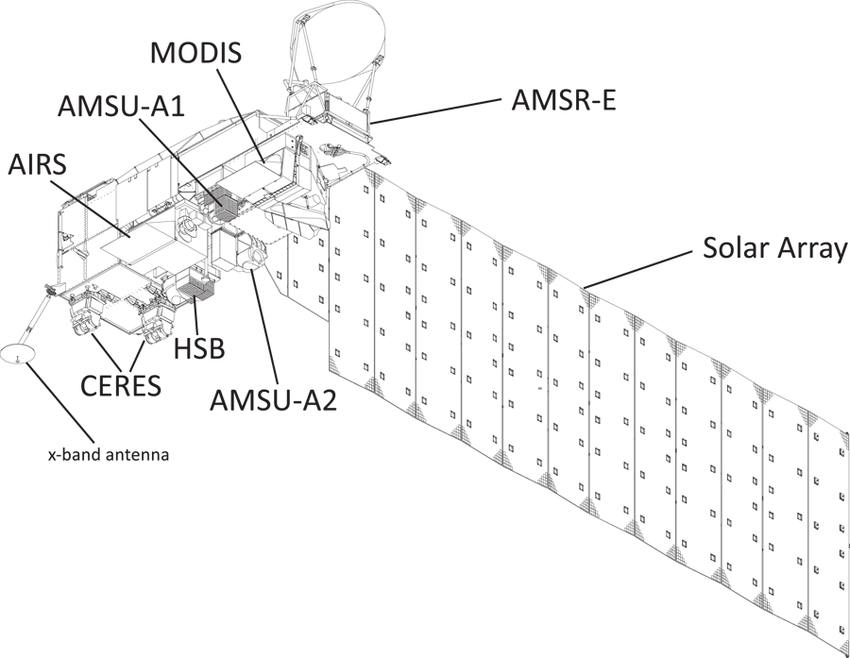
\includegraphics[width = 10cm]{Images/Schematic-of-the-Aqua-spacecraft-its-six-Earth-observing-instruments-12-panel-solar.png}
    \caption{Schematic of Aqua Instruments}
    \label{fig:squa-schematic}
\end{figure}

Additionally, the total mass of the satellite was 2,934 kg at launch. The mass distribution was 1,750 kg for the spacecraft structure, 1,082 kg for the instruments, and 102 kg for the propellant. Going into more detail, the individual mass of each of the instuments shown in Figure \ref{fig:squa-schematic} was also obtained. The MODIS had a mass of 229 kg. The AIRS had a mass of 177 kg. The AMSU-A had a mass of 91 kg. The HSB had a mass of 51 kg. The AMSR-E had a mass of 314 kg. Finally, the CERES had a mass of 50 kg per sensor of which there are two. It can be seen that with these instrument masses, their sum is 962 kg. Therefore, the mass of the overall system after both launch and deployment would have been 2814 kg. \cite{aqua_mass_sumaries} Even though the mass distribution and inertia properties of Aqua are not public information, by combining this information with Figure \ref{fig:squa-schematic}, a rough mass distribution and inertia properties such as the center of mass and moment of inertia can be obtained.

\subsubsection{Simplify spacecraft geometry, make assumptions on mass distribution, e.g. splitting it in its core parts, define body axes (typically related to geometry and payload), compute moments of inertia and full inertia tensor w.r.t. body axes. Show your calculations.}

A model of the satellite was generated with the geometry greatly simplified as shown in Figure \ref{fig:aquacad}. Each instrument listed in the previous section was approximated as a rectangular prism with a uniform mass distrubution corresopnding to the aforementioned instrument masses in Section \ref{sec:mission_info}. 


\begin{figure}[H]
    \centering
    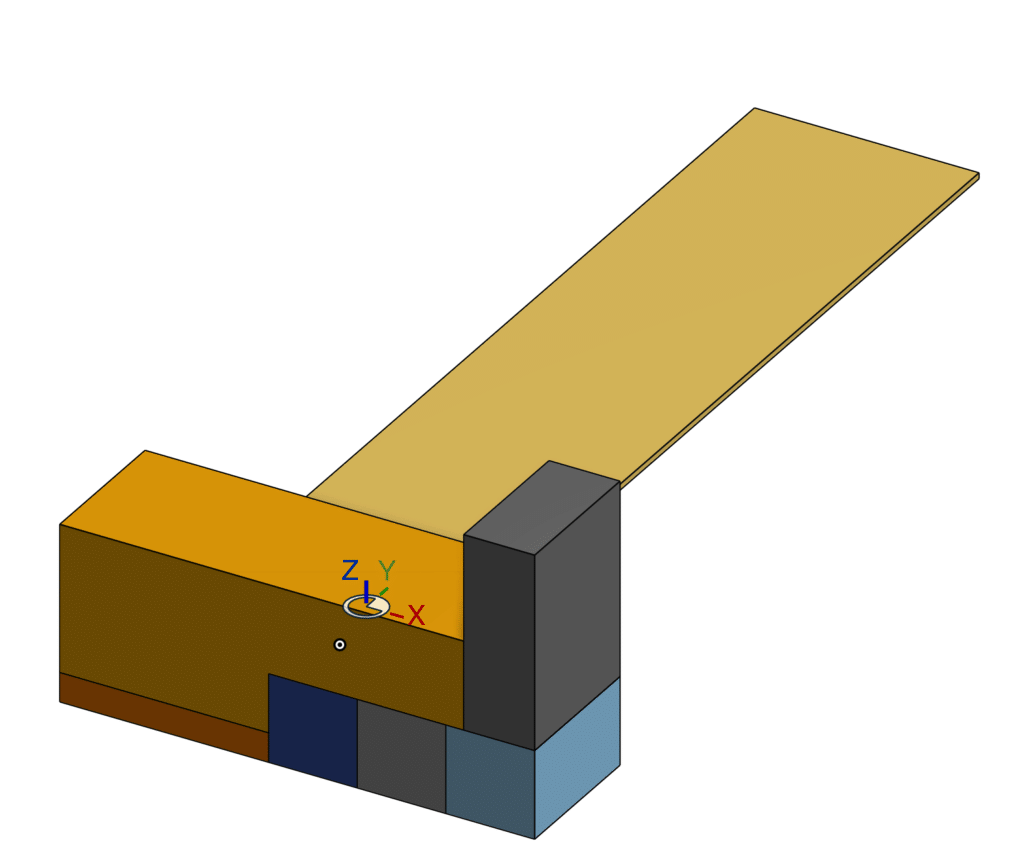
\includegraphics[width = 10cm]{Images/AquaSat-1.png}
    \caption{Simplified Aqua Model}
    \label{fig:aquacad}
\end{figure}

The location of the center of mass was calculated using Equation \ref{eq:center_mass} with distances measured from the lower-most corner oriented with the body coordinate system, whose orientation is  depicted in Figure \ref{fig:aquacad}. 

\begin{equation} \label{eq:center_mass}
    \vec{r} = \begin{bmatrix}
        \bar{x} & \bar{y} & \bar{z}
    \end{bmatrix}^T = \begin{bmatrix}
        \frac{\sum_{i=1}^N{m_i x_i}}{\sum_{i = 1}^N{m_i}} & \frac{\sum_{i=1}^N{m_i y_i}}{\sum_{i = 1}^N{m_i}} & \frac{\sum_{i=1}^N{m_i z_i}}{\sum_{i = 1}^N{m_i}}
    \end{bmatrix}^T
\end{equation}

The vector in this equation represents a position vector of the satellite's center of mass. The mass of each component in the satellite is denoted by $m_i$ where the position vector of each components center of mass has coordinates described as $\vec{r_i} = \begin{bmatrix}
    x_i & y_i & z_i
\end{bmatrix}^T$. The calculations were done using the component masses and locations tabulated below, which were pulled from the CAD model. The total mass along with the location of the satellite's center of mass is presented in the bottom row of Table \ref{tab:mass_props}. The mass of the chassis and solar panel were approximated by summing the non-instrument mass and propellant mass and uniformly distributing it between the two components.

\begin{table}[H]
    \centering
    \begin{tabular}{c|cccc}
    Component & $m_i$ [kg] & $x_i$ [m] & $y_i$ [m] & $z_i$ [m] \\ \hline
    MODIS     &    229   &    7.29   &   1.25    &   0.75    \\
    AMSU-A1   &     49  &    5.79   &    1.25   &   0.75    \\
    AMSU-A2    &    42   &    4.665   &   1.875    &  0.75   \\
    AIRS        &    177   &    4.29   &   0.625    &   0.75    \\
    HSB         &    51   &     3.915  &    1.875   &    0.75   \\
    CERES       &   100    &    1.77   &   1.25    &   0.25    \\
    AMSR-E      &    314   &    7.44   &    1.25   &   3.15    \\
    Chassis     &     1607  &    2.997   &   1.25    &    1.929   \\
    Solar Panel     &   245    &   4.02    &   9.6    &    2.25   \\ \hline
    Total       & 2184      & 4.059     & 1.958     & 1.804
    \end{tabular}
    \caption{Mass Properties and Distribution for Satellite Components}
    \label{tab:mass_props}
\end{table}

Following this, the moment of inertia for the satellite was computed. To compute this, first the moments of inertia of each component were taken about their own centers of mass. In general, the moment of inertia of a body is calculated using Equation \ref{eq:general_inertia}. Approximating each of the components as a rectangular prism, the moment of inertia about the centers of mass is found through using Equation \ref{eq:rect_inertia}, where $\rho$ is the mass density and $l_x$, $l_y$, and $l_z$ represent the lengths of each prism along the coordinate directions.

\begin{equation} \label{eq:general_inertia}
    \boldsymbol{I_{CM}} = \left[ \begin{array}{ccc}
     \int{(y^2 + z^2)}dm & \int{-  xy}dm & \int{-  xz}dm \\
\int{-  xy}dm &   \int{(x^2 + z^2)}dm & \int{-  yz}dm \\
\int{-  xz}dm & \int{-  yz}dm &  \int{(x^2 + y^2)}dm \\
    \end{array} \right]
\end{equation}

\begin{equation} \label{eq:rect_inertia}
    \boldsymbol{I_{CM}} = \left[ \begin{array}{ccc}
       \frac{1}{12}\rho l_x \left( l_y^3 l_z + l_z^3 l_y \right)  & 0 & 0 \\
         0  & \frac{1}{12}\rho l_y \left( l_x^3 l_z + l_z^3 l_x \right) & 0 \\
         0  & 0 &  \frac{1}{12}\rho l_z \left( l_x^3 l_y + l_y^3 l_x \right)
         \end{array} \right]
\end{equation}

Table \ref{tab:mass_props} shows the properties that were used to calculate the moment of inertias as well as the component-wise results. 

\begin{table}[H]
    \centering
    \begin{tabular}{c|ccccccc}
    Component & $\rho$ [kg/m\textsuperscript{3}] & $l_x$ [m] & $l_y$ [m] & $l_z$ [m] & $I_{xx}$ [kg m\textsuperscript{2}] & $I_{yy}$ [kg m\textsuperscript{2}] & $I_{zz}$ [kg m\textsuperscript{2}] \\ \hline
    MODIS       &    40.711    &   1.50    &   2.50     &  1.50     &  612.21      &  85.875      &   162.21     \\
    AMSU-A1     &    8.7111    &   1.50    &   2.50     &  1.50     &  34.708     &   18.375     &    34.708    \\
    AMSU-A2     &    29.867    &   0.75    &   1.25     &  1.50     &  13.344     &   9.814     &   7.438     \\
    AIRS        &    62.933    &   1.50    &   1.25     &  1.50     &  56.234     &   66.375     &  56.234      \\
    HSB         &    36.267    &   0.75    &   1.25     &  1.50     &  16.203     &   11.953     &  9.0310      \\
    CERES       &    22.599    &   3.54    &   2.50     &  0.50     &  54.167     &   106.51     &  156.51      \\
    AMSR-E      &    31.717    &   1.20    &   2.50     &  3.30     &  448.50     &   322.64     &  201.222      \\
    Solar Panel &    45.404    &   3.80    &   14.2    &   0.1    &    4117.0    &    295.00    &   4411.6     \\
    \end{tabular}
    \caption{Mass Properties and Distribution for Satellite Components}
    \label{tab:mass_props}
\end{table}

The chassis inertia had to be computed in a different manner using a composition of rectangles. The approach taken in this paper was to first take the inertia about a geometrically convenient point, then use the parallel axis theorem to determine the inertia about the center of mass of the chassis. The composition chosen was one where a larger rectangle of uniform density has from it a component of equivalent density subtracted. This composition is described in Table \ref{tab:composite_chassis}.

\begin{table}[H]
    \centering
    \begin{tabular}{c|ccccccc}
    Member  & $\rho$ & $l_x$ & $l_y$ & $l_z$ & $I_{xx}$ & $I_{yy}$ & $I_{zz}$ \\ \hline
    Prism 1 &   46.580     &   6.84    &   2.5    &   2.5    &  2074.3      &   8800.7     &   8800.7     \\
    Prism 2 &   -46.580     &  3.3     &   2.5    &   1.0    &  232.17      &   380.76     &   548.88     \\  
    \end{tabular}
    \caption{Mass Properties for Composite Chassis}
    \label{tab:composite_chassis}
\end{table}

Using the parallel axis theorem, seen in Equation \ref{eq:par_axis}, the moment of inertia of the composite shape about the center of mass of prism 1 along with the inertia about the center of mass of the object is shown in Table \ref{tab:chass_inertia}. In Equation \ref{eq:par_axis}, $\boldsymbol{I_P}$ is the inertia tensor about an arbitrary point P whose position relative to the center of mass is $\vec{r} = \begin{bmatrix} x & y & z \end{bmatrix}^T$.

\begin{equation} \label{eq:par_axis}
    \boldsymbol{I_{P}} = \boldsymbol{I_{CM}} + m \left[ \begin{array}{ccc}  (y^2 + z^2) & -  xy & -  xz \\ 
    -  xy &   (x^2 + z^2) & -  yz \\
-  xz & -  yz &  (x^2 + y^2) \\ \end{array} \right]
\end{equation}


\begin{table}[H]
    \centering
    \begin{tabular}{c|cccccc}
    Reference Point   & $I_{xx}$ & $I_{yy}$ & $I_{zz}$ & $I_{xy}$ & $I_{xz}$ & $I_{yz}$ \\ \hline
    Center of Prism 1 & 1625.9   & 7000     & 7047.9   & 0        & -510.10  & 0        \\
    Center of Mass    & 1574.2   & 6660.3   & 6760.0   & 0        & -632.12  & 0       
    \end{tabular}
    \caption{Inertia Tensors of Chassis about Intermediate Reference and Center of Mass}
    \label{tab:chass_inertia}
\end{table}

Now applying parallel axis theorem to each component, Aqua's inertia tensor about its own center of mass is shown in Table \ref{tab:total_ineretia}.

\begin{table}[H]
\centering
\begin{tabular}{c|cccccc}
                     & $I_{xx}$ & $I_{yy}$ & $I_{zz}$ & $I_{xy}$ & $I_{xz}$ & $I_{yz}$ \\ \hline
Total Inertia Tensor & 23745    & 17560    & 36065    & 93.907   & -1267.1  & -967.50 
\end{tabular}
\caption{Total Inertial Tensor about Satellite Center of Mass Directed along Body Axes}
\label{tab:total_ineretia}
\end{table}

Below is the script written to perform all of the above calculations.

\begin{lstlisting}
clc, clear 
close all

%% Instrument Moments of Inertia

instruments = {'MODIS', 'AMSU-A1', 'AMSU-A2', 'AIRS', 'HSB', 'CERES', 'AMSR-E'};
lxs = [1.5, 1.5, 0.75, 1.5, 0.75, 3.54, 1.2];
lys = [2.5, 2.5, 1.25, 1.25,1.25, 2.5, 2.5];
lzs = [1.5, 1.5, 1.5, 1.5, 1.5, 0.5, 3.3];
ms = [229, 49, 42, 177, 51, 100, 314];
Vs = lxs.*lys.*lzs;
rhos = ms./Vs;
Icms = zeros([3 3 7]);

for i = 1:7
    Icms(:,:,i) = rectInertia(lxs(i),lys(i),lzs(i),rhos(i));
end
%% Chassis

V = 34.5;
Vsub = 3.3*2.5*1;
Vt = V + Vsub;
m = 1607;
rho = m/V;

It = rectInertia(6.84, 2.5, 2.5, rho);

Is = rectInertia(3.3,2.5,1,rho);

xbar = 1.77;
ybar = 0;
zbar = -0.75;

Is = parallelAxis(Is,xbar,ybar,zbar,rho,Vsub);

Ichassis = It - Is;

xbart = 3.42;
ybart = 1.25;
zbart = 1.75;

xbars = xbart + xbar;
ybars = ybart + ybar;
zbars = zbart + zbar;

xbarc = (Vt*xbart - Vsub*xbars)/V
ybarc = (Vt*ybart - Vsub*ybars)/V
zbarc = (Vt*zbart - Vsub*zbars)/V

xtild = xbart - xbarc;
ytild = ybart - ybarc;
ztild = zbart - zbarc;

Ichassis = parallelAxis(Ichassis, xtild, ytild, ztild, -rho, V)

%% Solar Panel

lx = 3.8;
ly = 14.2;
lz = 0.1;
V = lx*ly*lz;
m = 245;
rho = m/V;

Isolar = rectInertia(lx,ly,lz,rho);

%% COM

ms = [ms, 1607, 245];
Vs = [Vs, 34.5, 5.396];
rhos = ms./Vs;
Icms = cat(3, Icms, Ichassis, Isolar);

xis = [7.29, 5.79, 4.665, 4.29, 3.915, 1.77, 7.44, xbarc, 8.04/2];
yis = [1.25, 1.25, 1.875, 0.625, 1.875, 1.25, 1.25, ybarc, 9.6];
zis = [0.75, 0.75, 0.75, 0.75, 0.75, 0.25, 3.15, zbarc, 2.25];

xyzBar = centerMass(ms, xis, yis, zis);

%% Total Moment of Inertia

% xis(8) = 6.84/2;
% zis(8) = 1.75;

x0s = xis - xyzBar(1);
y0s = yis - xyzBar(2);
z0s = zis - xyzBar(3);

Itotal = zeros([3 3]);

for i=1:9
    Itotal = Itotal + parallelAxis(Icms(:,:,i), x0s(i), y0s(i), z0s(i), rhos(i), Vs(i));
end

%% Functions

function I = rectInertia(lx, ly, lz, rho)

% rho = m/V;

I = zeros([3 3]);

% Ixy = 0, Iyz = 0, Ixz = 0;

Ixx = (1/12).*rho.*lx.*(ly.^3.*lz + lz.^3.*ly);
Iyy = (1/12).*rho.*ly.*(lx.^3.*lz + lz.^3.*lx);
Izz = (1/12).*rho.*lz.*(lx.^3.*ly + ly.^3.*lx);

I(1,1) = Ixx;
I(2,2) = Iyy;
I(3,3) = Izz;

end

function I = parallelAxis(Icm, x, y, z, rho, V)

Iplus = rho*V*[y^2 + z^2, -x*y, -x*z;
            -x*y, x^2 + z^2, -y*z;
            -x*z, -y*z, x^2 + y^2];

I = Icm + Iplus;

end

function xyzBar = centerMass(ms, xs, ys, zs)

xbar = sum(xs.*ms)/sum(ms);
ybar = sum(ys.*ms)/sum(ms);
zbar = sum(zs.*ms)/sum(ms);

xyzBar = [xbar, ybar, zbar];

end
\end{lstlisting}

\subsubsection{Discretize your spacecraft through its outer surfaces (geometry). Develop a Matlab/Simulink function to handle barycenter (geometry, no mass distribution) coordinates, size, and unit vectors normal to each outer surface of the spacecraft in body frame. You can list all this information in a Matrix. }

Descriptions of all surfaces through barycenter coordinates, surfaces normal vectors, and surface areas are recorded below in Table \ref{tab:surface_data} with the corresponding surfaces labeled in Figure \ref{fig:surface_labels}. 

% Please add the following required packages to your document preamble:
% \usepackage{multirow}
\begin{table}[H]
\centering
\begin{tabular}{c|ccc|ccc|c}
        & \multicolumn{3}{c|}{Surface Normal Vector} & \multicolumn{3}{c|}{Centroid Coordinates} & \multirow{2}{*}{Area [m\textsuperscript{2}]} \\ \cline{2-7}
Surface & $n_x$        & $n_y$        & $n_z$        & $x$ [m]  & $y$ [m]  & $z$ [m] &                                                                   \\ \hline
1       & 0            & -1           & 0            & 4.30         & 0            & 1.70        & 26.28                                                             \\
2       & 1            & 0            & 0            & 8.04         & 1.25         & 2.40        & 12.00                                                             \\
3       & 0            & 0            & 1            & 7.44         & 1.25         & 4.80        & 3.000                                                             \\
4       & -1           & 0            & 0            & 0            & 1.25         & 1.5         & 7.500                                                             \\
5       & 0            & 0            & 1            & 3.42         & 1.25         & 3.00        & 17.10                                                             \\
6       & 0            & 0            & 1            & 4.02         & 9.60         & 2.30        & 53.96                                                             \\
7       & 0            & 0            & -1           & 4.02         & 9.60         & 2.30        & 53.96                                                             \\
8       & -1           & 0            & 0            & 6.84         & 1.25         & 3.90        & 4.500                                                             \\
9       & 0            & 1            & 0            & 4.30         & 0            & 1.70        & 26.28                                                             \\
10      & 0            & 0            & -1           & 4.02         & 1.25         & 0           & 20.10                                                            
\end{tabular}
\caption{Normal Vectors, Barycenter Coordinates, and Surface Area for All Outer Surfaces}
\label{tab:surface_data}
\end{table}

\begin{figure}[H]
    \centering
    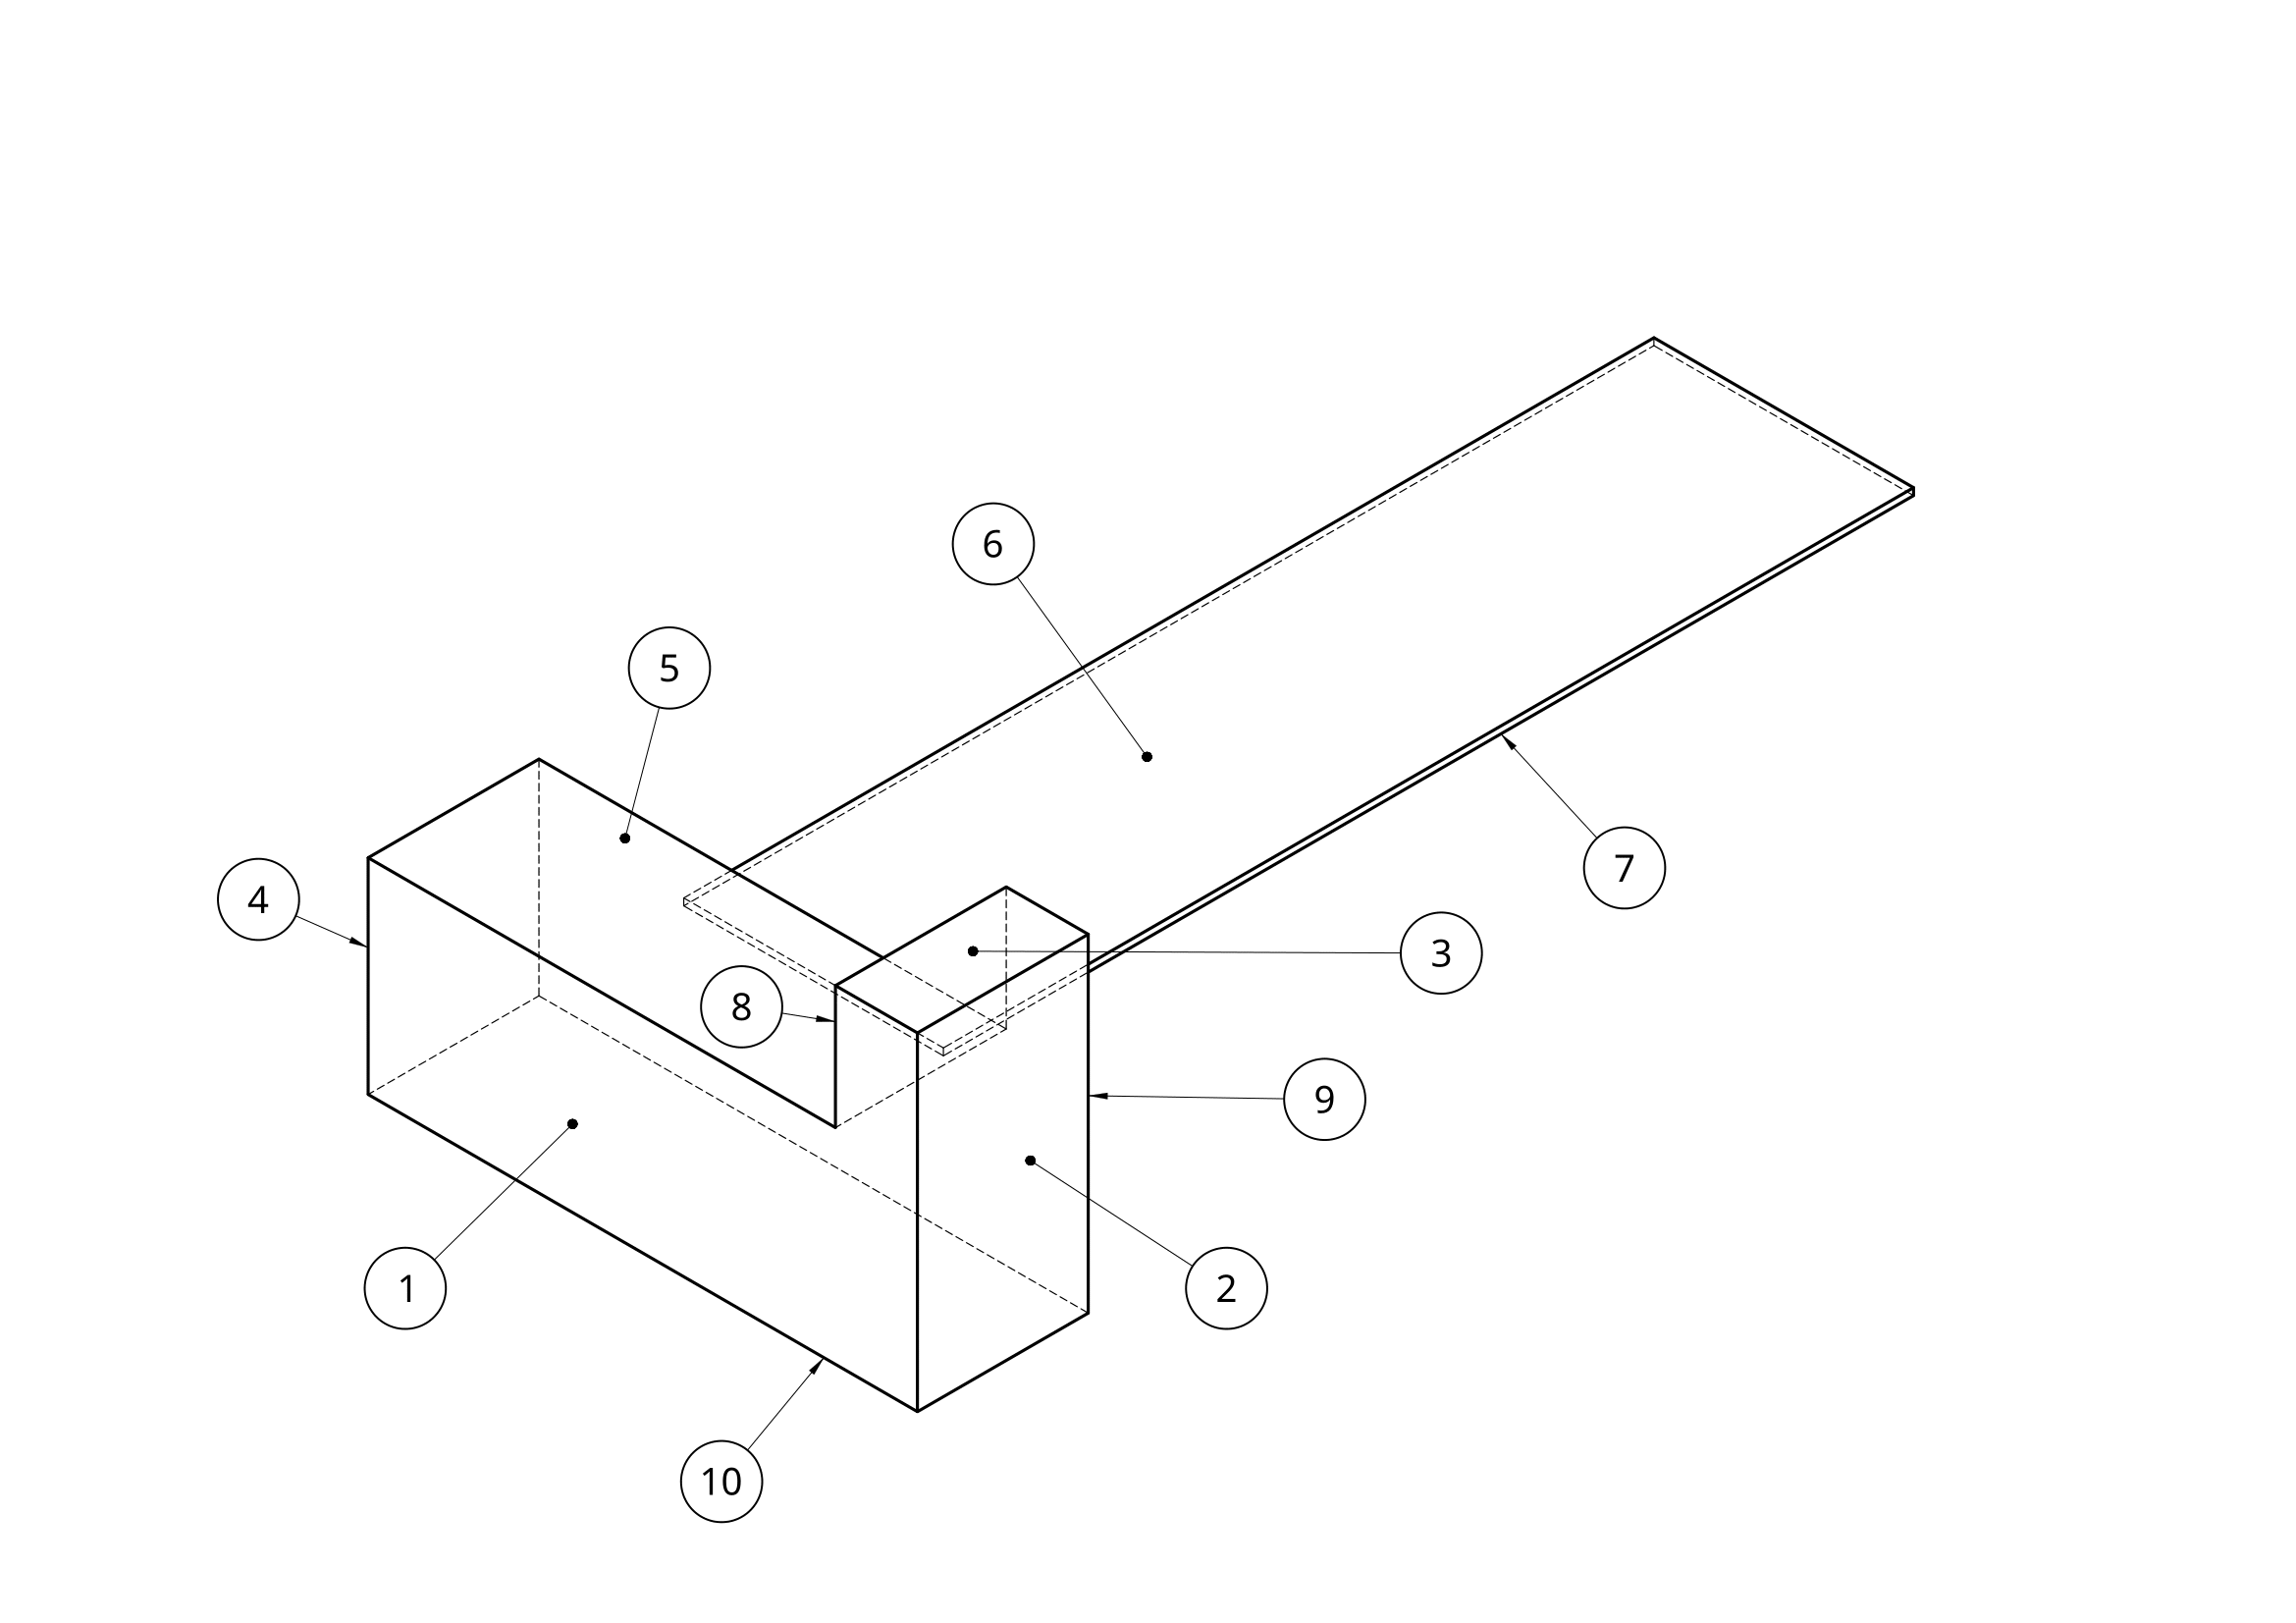
\includegraphics[width = 14cm]{Images/AquaSurfaces.png}
    \caption{Schematic of Aqua's Outer Surfaces Discretized and Labeled}
    \label{fig:surface_labels}
\end{figure}

The script that was used to store this data is seen below:


\begin{lstlisting}
clc, clear
close all

A1s = [6.84*3, 1.2*4.8].';
P1s = [6.84/2, 0, 3/2;
        6.84 + 1.2/2, 0, 4.8/2];
[A1, P1] = cent(A1s, P1s);
A9 = A1; P9 = P1;
N1 = [0 -1 0]; N9 = -N1;

A2 = 4.8*2.5;
P2 = [8.04, 2.5/2, 4.8/2];
N2 = [1 0 0];

A3 = 1.2*2.5;
P3 = [6.84 + 1.2/2, 2.5/2, 4.8];
N3 = [0 0 1];

A4 = 2.5*3;
P4 = [0 2.5/2, 3/2];
N4 = [-1 0 0];

A5 = 2.5*6.84;
P5 = [6.84/2, 2.5/2, 3];
N5 = [0 0 1];

A6 = 14.2*3.8; A7 = A6;
P6 = [4.02, 9.6, 2.3]; P7 = P6;
N6 = [0 0 1]; N7 = -N6;

A8 = 2.5*1.8;
P8 = [6.84, 2.5/2, 3 + 1.8/2];
N8 = [-1 0 0];

A10 = 8.04*2.5;
P10 = [8.04/2, 2.5/2, 0];
N10 = [0 0 -1];

N = [N1;N2;N3;N4;N5;N6;N7;N8;N9;N10];
A = [A1;A2;A3;A4;A5;A6;A7;A8;A9;A10];
P = [P1;P2;P3;P4;P5;P6;P7;P8;P9;P10];

%% Centroid Function
function [Ai, Pi] = cent(As, Ps)

Ai = sum(As);

x = sum(Ps(:,1).*As)./Ai;
y = sum(Ps(:,2).*As)./Ai;
z = sum(Ps(:,3).*As)./Ai;

Pi = [x, y, z];

end
\end{lstlisting}
\section{\Large PROBLEM SET 2}
\subsection{Problem 2}

\subsubsection{Define orbit initial conditions and make sure you can propagate the orbit of the satellite over multiple orbits using either a Keplerian propagator or a numerical integration scheme.}

The orbit initial conditions were chosen to closely replicate those of the Aqua satellite. The orbit is sun-synchronous, has an eccentricity of almost zero, and has an altitude similar to that of Aqua.

\begin{center}
    a = 7080.6 km \\
    e = 0.0000979 \\
    i = 98.2\degree \\
    $\omega$ = 120.4799\degree \\
    $\Omega$ = 95.2063\degree \\
    $\nu$ = 0\degree
\end{center}

To propagate the orbit, these orbital elements were first converted to the initial position and velocity in the Earth centered Inertial (ECI) frame. The ECI frame is defined such that it doesn't rotate with Earth's surface. The x-axis points in the direction of the vernal equinox (the ascending node of the sun), the z-axis points towards the north pole, and the y-axis completes the triad. To initially propagate the orbit and serve as a point of reference, Simulink was used to sweep the mean anomaly over a given time span and time steps and calculate the position in the ECI frame at each time step. The Simulink model is shown below in Figure \ref{fig:simulink-prop}.

\begin{figure}[H]
    \centering
    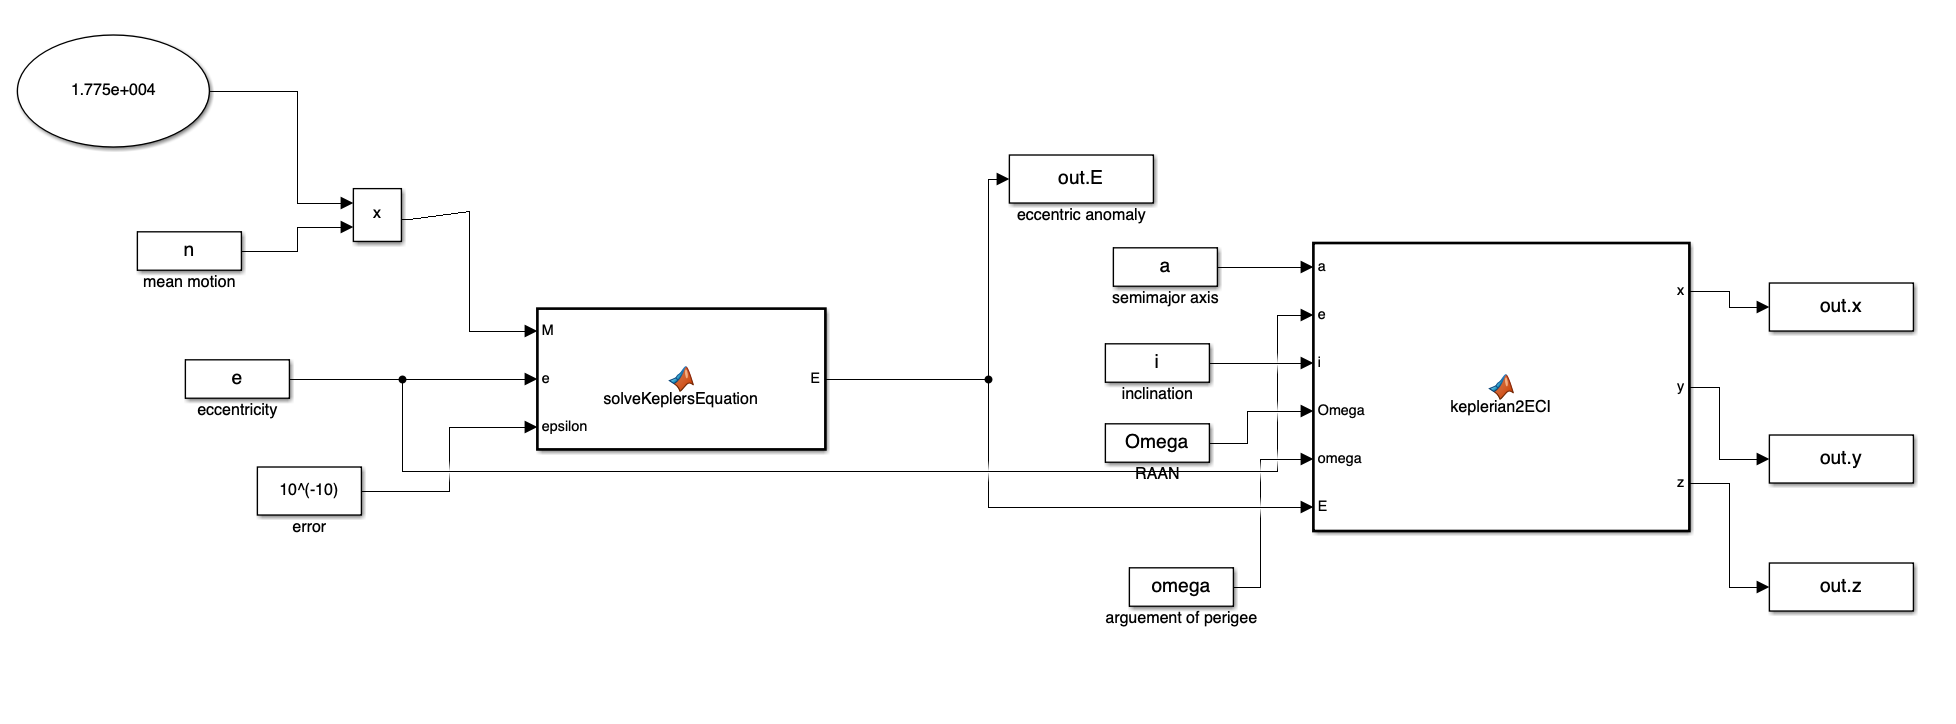
\includegraphics[width = 15.5cm]{Images/simulink_prop.png}
    \caption{Simulink Model for Keplerian Propagator}
    \label{fig:simulink-prop}
\end{figure}

The Keplerian propagator was then used to plot the orbit for a time span roughly equal to three orbital periods. The resulting orbit along with a spherical model of Earth is shown below in Figure \ref{fig:kep_orbit}.

\begin{figure}[H]
    \centering
    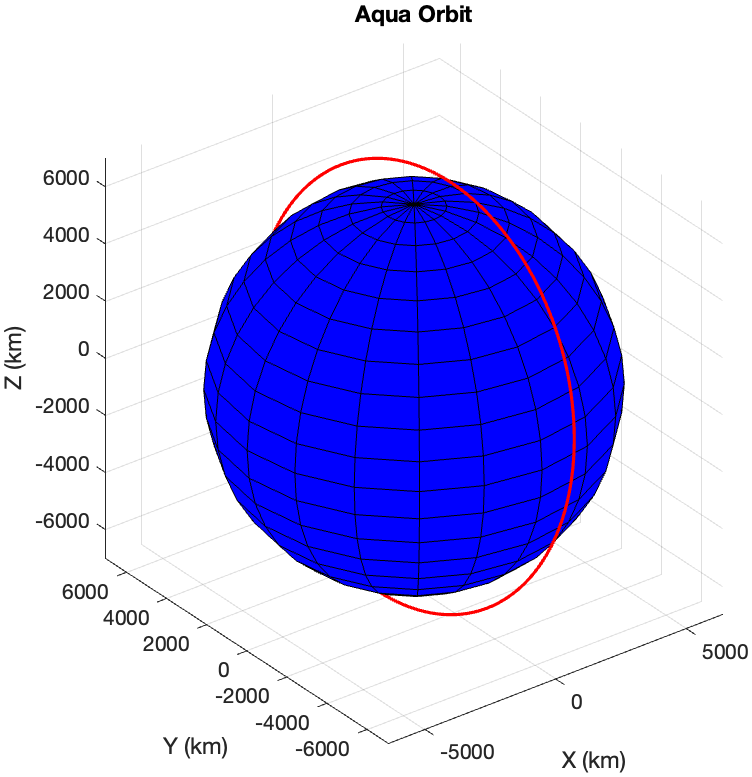
\includegraphics[width = 8.5cm]{Images/aqua_orbit_kepler.png}
    \caption{Aqua Orbit for Keplerian Propagator}
    \label{fig:kep_orbit}
\end{figure}

The Matlab function that was used for the Keplerian propagator can also be seen here.

\lstinputlisting{code}


\subsubsection{In general the body axes are not the principal axes. Identify principal axes through the eigenvector/eigenvalue problem discussed in class and compute the rotation matrix from body to principal axes.} \label{sec:principal_inertia_def_and_calc}

To resolve an inertia tensor $\boldsymbol{I_{CM}}$ to a diagonal matrix of principal moments of inertia, there must exist a matrix, $\boldsymbol{A}$ such that the Equation \ref{eq:principal_moments} holds, where $\boldsymbol{I_{CM}'}$ is the principal moment of inertia tensor about the center of mass.

\begin{equation} \label{eq:principal_moments}
    \boldsymbol{I_{cm} A} = \boldsymbol{A I_{CM}'} 
\end{equation}

It can be seen that the principal moments of inertia are the eigenvalues of the inertia tensor and that the matrix $\boldsymbol{A}$ is a matrix whose columns are the right eigenvectors or the inertia tensor. For the AQUA spacecraft, the results that follow are shown below.

\begin{equation*}
    \boldsymbol{I_{CM}'} = \begin{bmatrix}
        17510 & 0 & 0 \\
        0 & 23616 & 0 \\
        0 & 0 & 36245
    \end{bmatrix} \text{kg} \cdot \text{m}^2
\end{equation*}

\begin{equation*}
    \boldsymbol{A} = \begin{bmatrix}
            0.0045  &  0.9949 &  -0.1011 \\
            -0.9986  & -0.0007  & -0.0520 \\
            -0.0518  &  0.1012  &  0.9935
    \end{bmatrix}
\end{equation*}

\subsubsection{At this stage you should have a simple 3D model of your spacecraft including geometry and mass properties of each element. This includes at least two coordinate systems, body and principal axes respectively, and the direction cosine matrix between them. Plot axes of triads in 3D superimposed to spacecraft 3D mode}

The body axes of the spacecraft are seen plotted in Figure \ref{fig:aquacad}. The principal inertia axes are seen plotted in Figure \ref{fig:aquacad_principal}.

\begin{figure}[H]
    \centering
    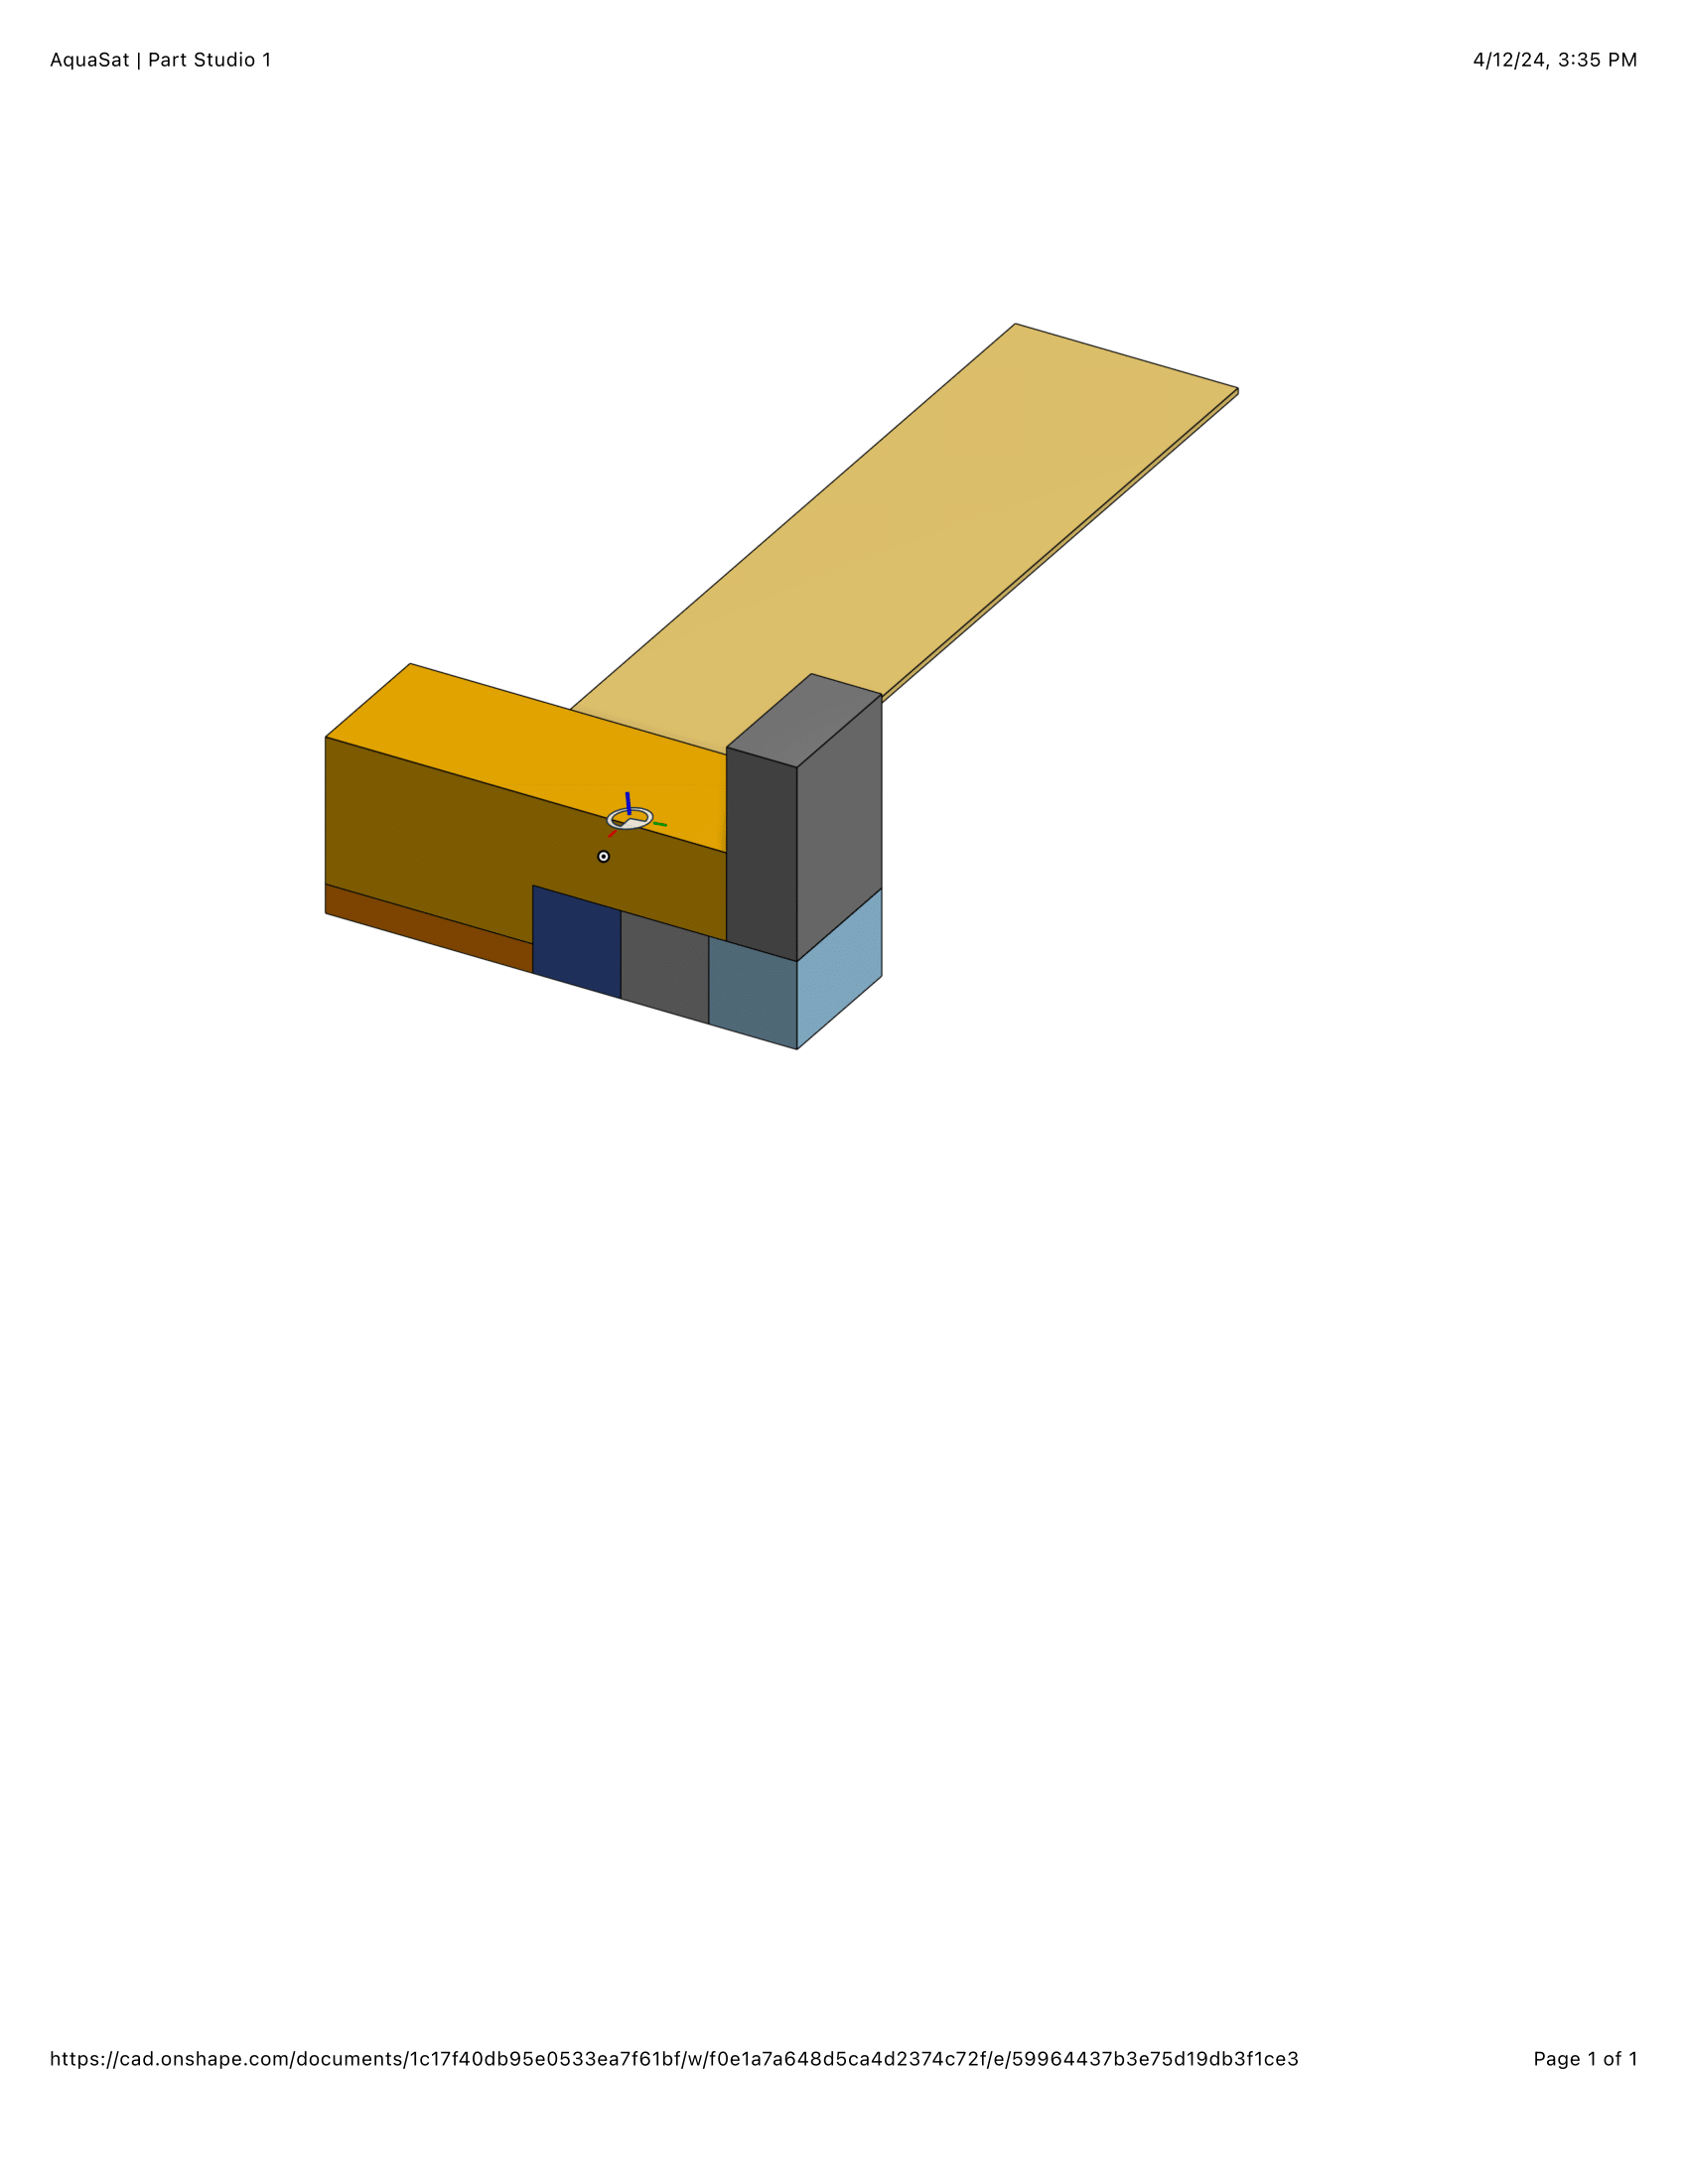
\includegraphics[width = 10cm]{Images/AquaSat_PrincipalAxes.png}
    \caption{Simplified Aqua Model with Principal Axes}
    \label{fig:aquacad_principal}
\end{figure}

\subsubsection{Program Euler equations in principal axes (e.g. in Matlab/Simulink). No external torques.}

The following Simulink model utilizing a MATLAB function (both in Figure \ref{fig:euler_prop_model}) takes in an initial rotational velocity vector and simulates the physics of the current AQUA model about the principal axes of inertia.

\begin{figure}[H]
    \centering
    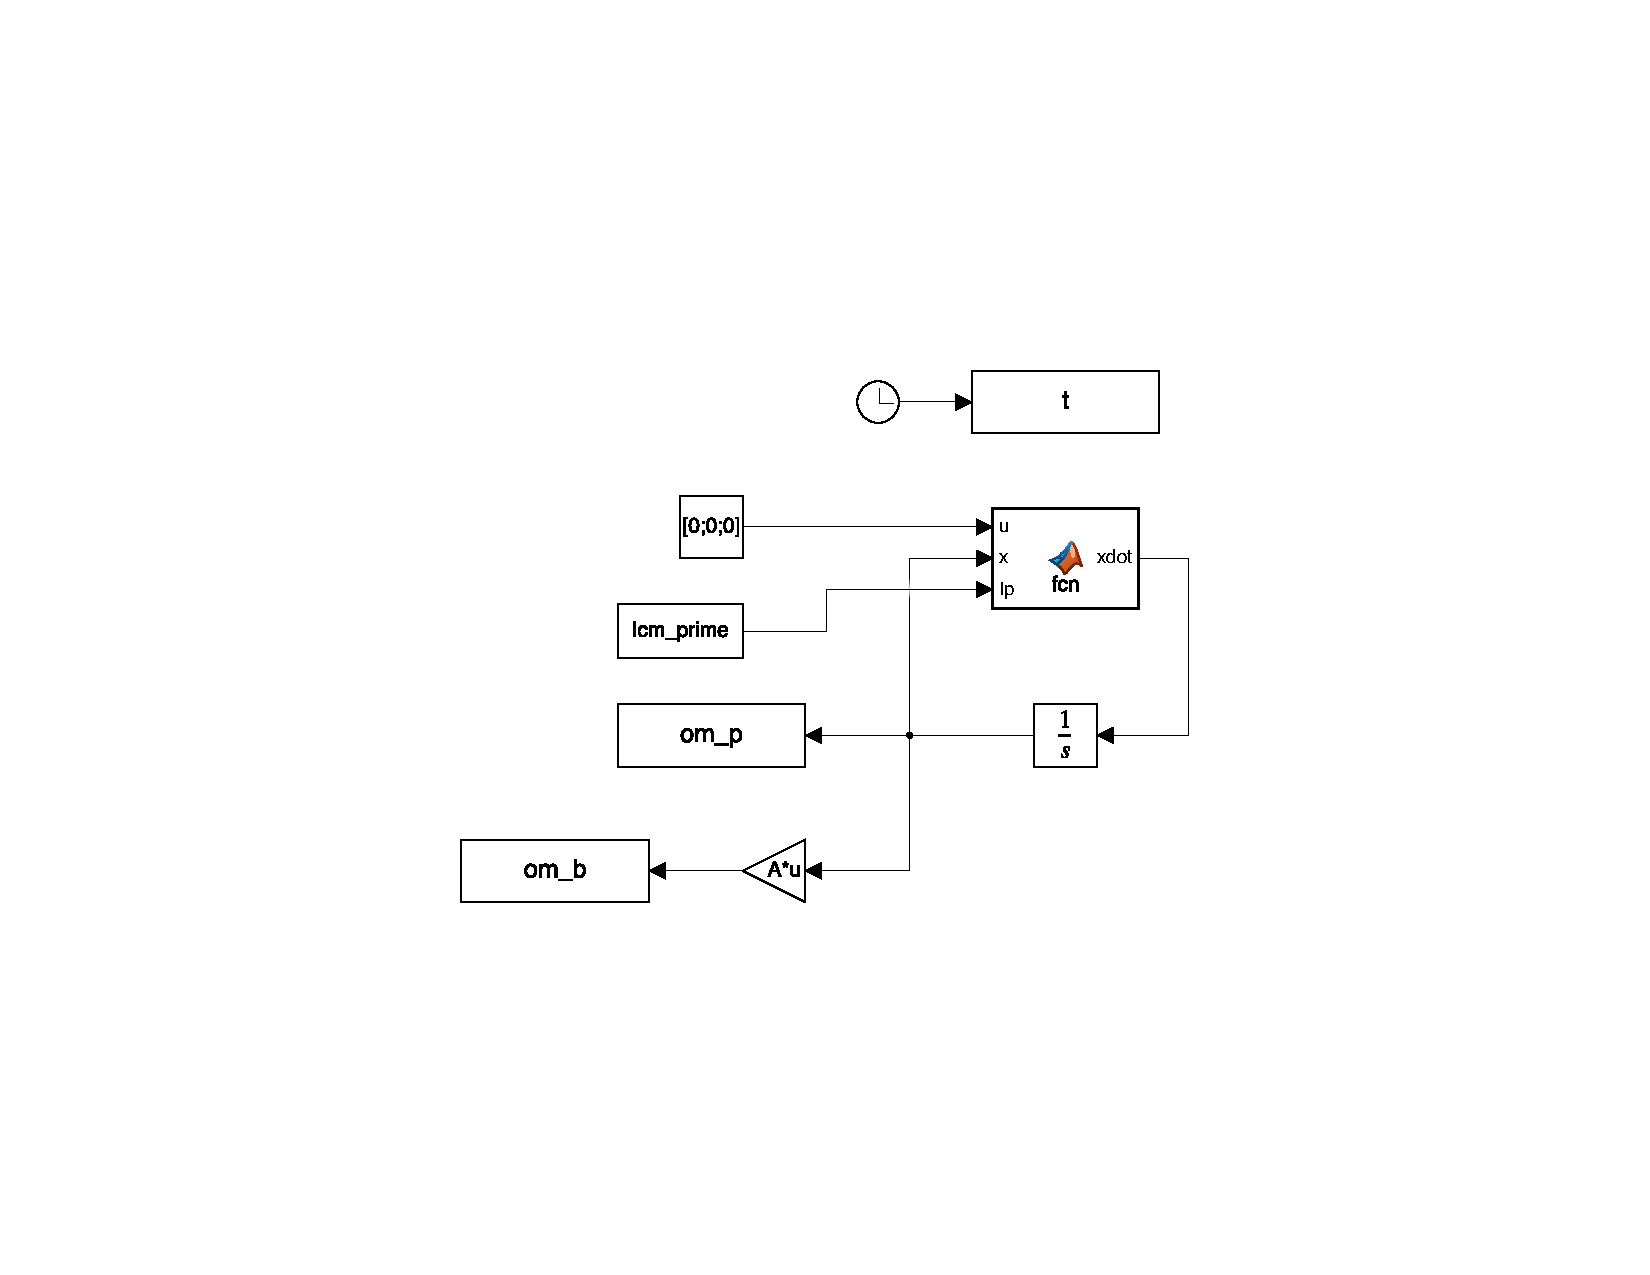
\includegraphics[trim={5cm 5cm 5cm 5cm},clip,width = 15cm]{Images/eulerPropagate.pdf}
\end{figure}

\begin{figure} [H]
    \centering
    \begin{lstlisting}
function xdot = fcn(u,x,Ip)

xdot = zeros(size(x));


Mx = u(1);
My = u(2);
Mz = u(3);

omx = x(1);
omy = x(2);
omz = x(3);

Ix = Ip(1,1);
Iy = Ip(2,2);
Iz = Ip(3,3);

wxdot = (1/Ix)*(Mx - (Iz - Iy)*omy*omz);
wydot = (1/Iy)*(My - (Ix - Iz)*omz*omx);
wzdot = (1/Iz)*(Mz - (Iy - Ix)*omx*omy);

xdot(1) = wxdot;
xdot(2) = wydot;
xdot(3) = wzdot;

end
    \end{lstlisting}
    \caption{Euler Propagation Simulink Model}
    \label{fig:euler_prop_model}
\end{figure}


\subsubsection{Numerically integrate Euler equations from arbitrary initial conditions ($\boldsymbol{\omega < 10^{\circ}/s}$, $\boldsymbol{\omega_i \neq 0}$). Multiple attitude revolutions.}

Given an initial condition of $\vec{\omega}_0 = \begin{bmatrix}
    -7 & 2 & 5
\end{bmatrix}^T {}^{\circ}/s$, gyroscopic coupling causes a periodic oscillation in the angular velocity vector represented in a body fixed axis frame. In this instance in particular, the simulation results shown in \ref{fig:sim_omegas} follows this evolution in the principal frame.

\begin{figure}[H]
    \centering
    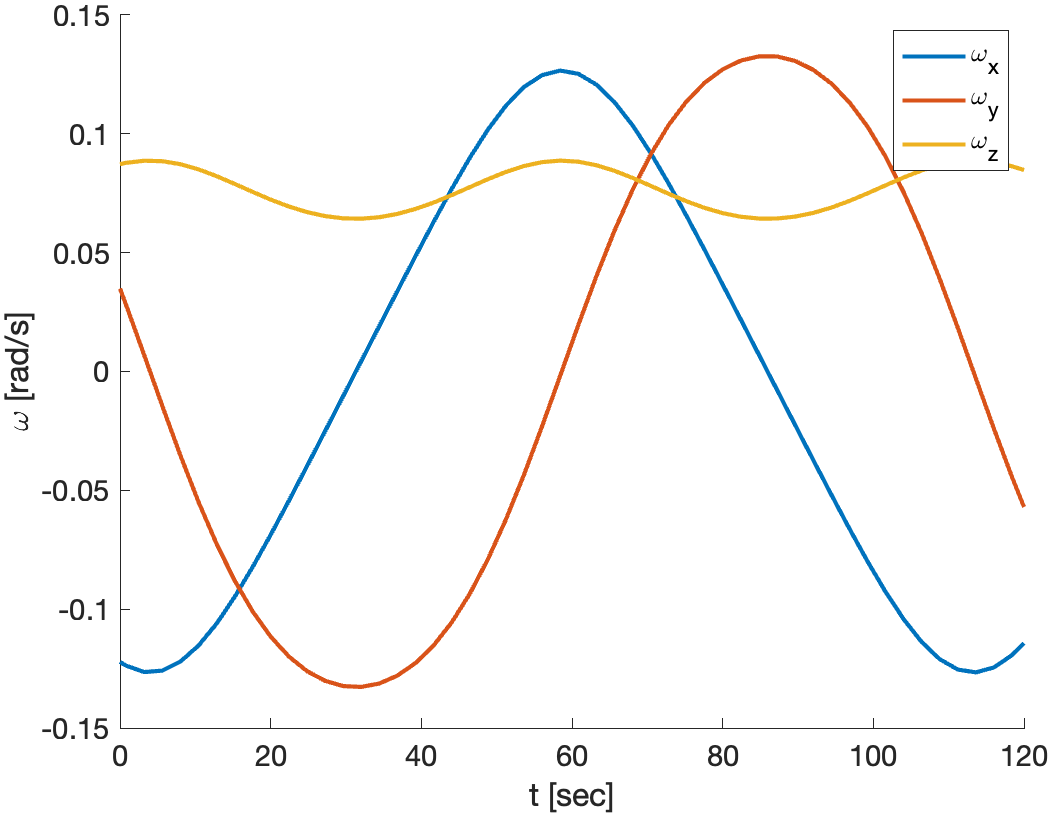
\includegraphics[width = 10cm] {Images/omega_prop_random.png}
    \caption{Angular Velocity Vector Components Evolving in the Body Fixed Principally Oriented Frame}
    \label{fig:sim_omegas}
\end{figure}

\subsubsection{Plot rotational kinetic energy and momentum ellipsoids in 3D (axis equal) corresponding to chosen initial conditions. Verify that semi-axis of ellipsoids corresponds to theoretical values} \label{sec:ellipsoid_definitions}

The angular momentum and rotational kinetic energy of a rigid body is computed using Equations \ref{eq:ang_mom} and \ref{eq:rot_KE} respectively, where $\vec{L}$ and $T$ are the momentum vector and energy, and the angular velocity vector in the principally oriented frame is described as $\vec{\omega} = \begin{bmatrix} \omega_x & \omega_y & \omega_z \end{bmatrix}^T$. 

\begin{equation} \label{eq:ang_mom}
    \vec{L} = \boldsymbol{I_{CM}'}\vec{\omega} = I_x \omega_x + I_y \omega_y + I_z \omega_z
\end{equation}

\begin{equation} \label{eq:rot_KE}
    T = \vec{\omega} \cdot \vec{L} = I_x \omega_x^2 + I_y \omega_y + I_z \omega_z^2
\end{equation}

These quantities are both conserved, so the satellite's angular velocity must always take on a vector value that yields the same momentum magnitude and kinetic energy as the initial conditions. With the initial conditions given above, the magnitude of angular momentum is 3906.4 kg m/s and the kinetic energy is 283.08 J. With not much manipulation, these relations can be shown to be equivalent to Equations \ref{eq:mom_ellipse} and \ref{eq:energy_ellipse} respectively, where L is the magnitude of the angular momentum vector.  

\begin{equation} \label{eq:mom_ellipse}
    \frac{\omega_x^2}{(L/I_x)^2} + \frac{\omega_y^2}{(L/I_y)^2} + \frac{\omega_z^2}{(L/I_z)^2} = 1
\end{equation}

\begin{equation} \label{eq:energy_ellipse}
    \frac{\omega_x^2}{2T/I_x} + \frac{\omega_y^2}{2T/I_y} + \frac{\omega_z^2}{2T/I_z} = 1
\end{equation}

By inspection, the form of these equations is that of an ellipsoid. Therefore, if the Cartesian coordinates are chosen such that the x,y, and z components of the angular velocity lie along the x,y, and z axes, the tip of the angular velocity vector plotted on these axes will lie on the surface of these ellipsoids. The momentum ellipsoid is plotted along with its semi-axis lengths is plotted in Figure \ref{fig:momentum_axis_verification}. The same is done for the energy ellipsoid in Figure \ref{fig:energy_axis_verification}

\begin{figure}[H]
    \centering
    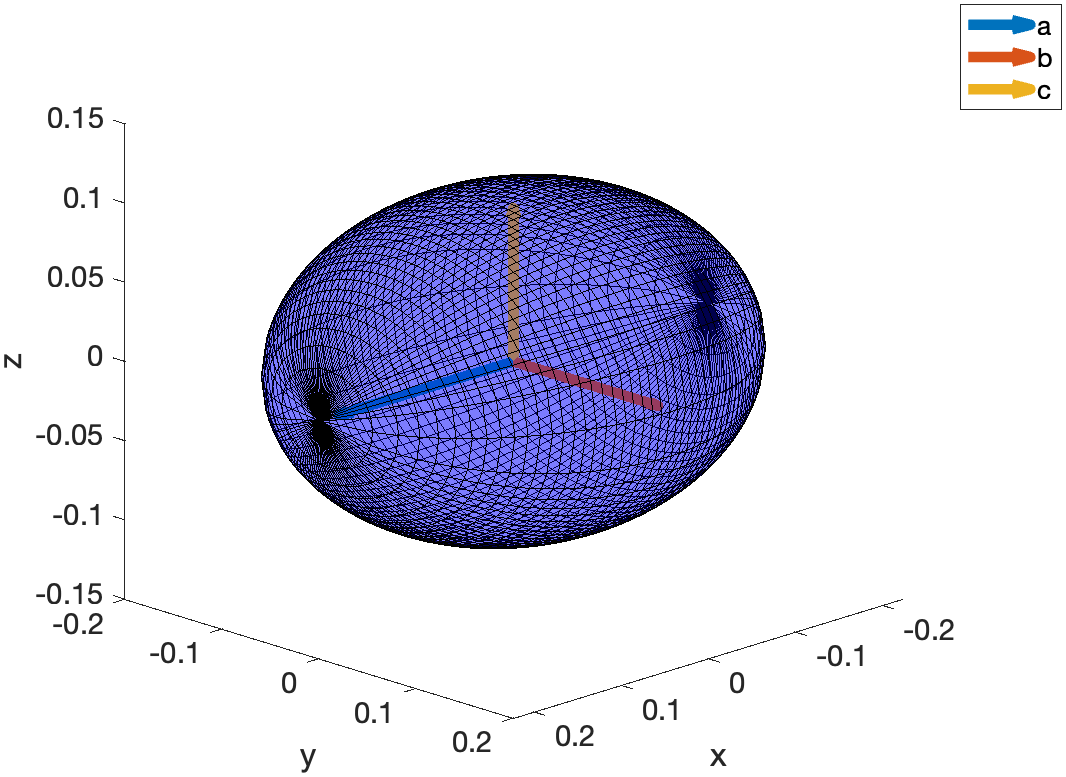
\includegraphics[width = 10cm]{Images/momentum_axes_random.png}
    \caption{Momentum Ellipsoid and Semi-Axis Lengths}
    \label{fig:momentum_axis_verification}
\end{figure}

\begin{figure}[H]
    \centering
    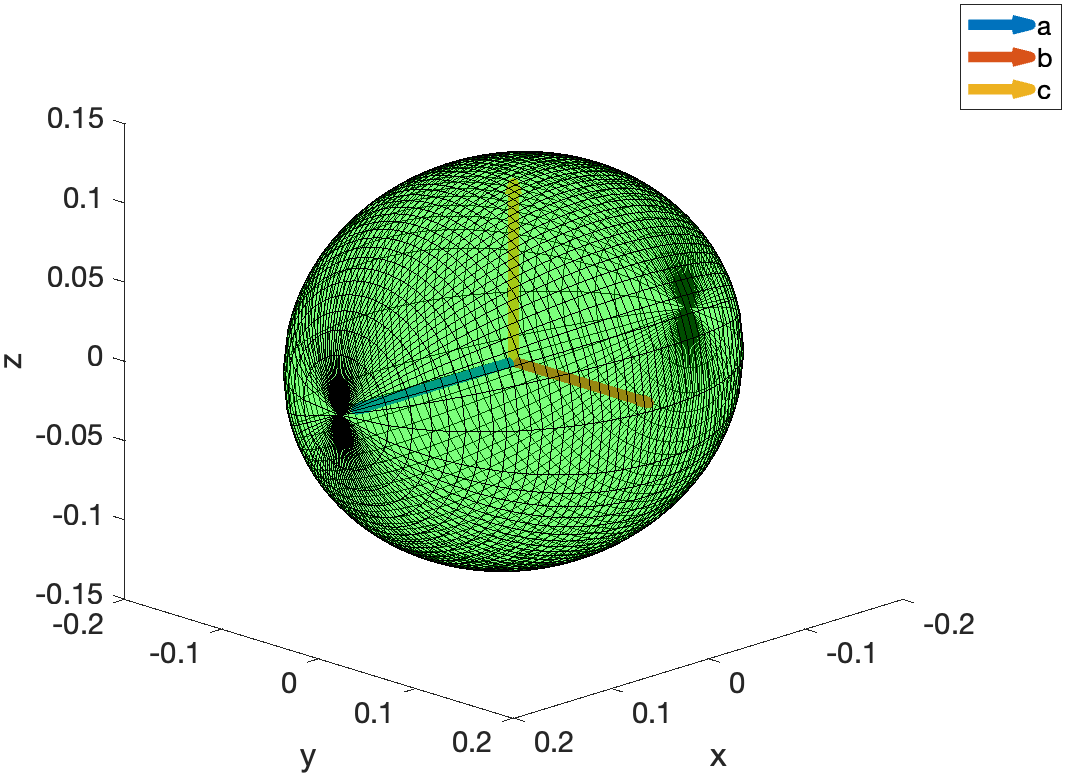
\includegraphics[width = 10cm]{Images/energy_axes_random.png}
    \caption{Energy Ellipsoid and Semi-Axis Lengths}
    \label{fig:energy_axis_verification}
\end{figure}

\subsubsection{Plot polhode in same 3D plot. Verify that it is the intersection between the ellipsoid}

Following that the angular velocity in a Cartesian plot must lie along the surface of both ellipsoids described in Section \ref{sec:ellipsoid_definitions}, it follows that the vector would be restricted to the intersection of the two ellipsoids. The curve that this vector traces is called the polhode, and the simulated results of this curve can be seen in Figure \ref{fig:ellipsoid_super_plot}, over-plotted with the momentum and energy ellipsoids. This curve matches the expected behavior in that it clearly traces the intersection between the momentum and energy ellipsoids. 

\begin{figure}[H]
    \centering
    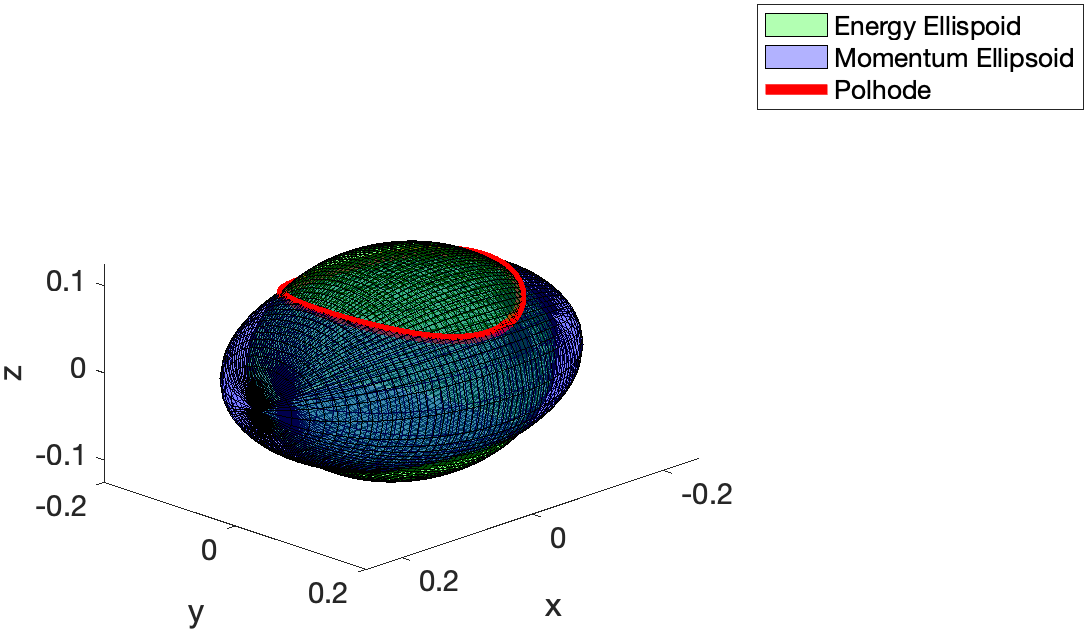
\includegraphics[width = 12cm] {Images/ellipsoid_polhode_random.png}
    \caption{Momentum and Energy Ellipsoids and Polhode Curve Plotted in 3D on Principally Aligned Coordinate Axes}
    \label{fig:ellipsoid_super_plot}
\end{figure}

\subsubsection{Plot polhode in three 2D planes identified by principal axes (axis equal). Verify that shapes of resulting conic sections correspond to theory.}

Figure \ref{fig:2d_polhode} shows the planar projections of the polhode curve along the labeled axes. In theory, these curves should be described by Equations \ref{eq:polhode1}, \ref{eq:polhode2}, and \ref{eq:polhode3}. 

\begin{equation} \label{eq:polhode1}
    (I_y - I_x)I_y \omega_y^2 + (I_z - I_x)I_z \omega_z^2 = L^2 - 2TI_x
\end{equation}

\begin{equation} \label{eq:polhode2}
    (I_x - I_y)I_x \omega_x^2 + (I_z - I_y)I_z \omega_z^2 = L^2 - 2TI_y
\end{equation}

\begin{equation} \label{eq:polhode3}
    (I_x - I_z)I_x \omega_x^2 + (I_y - I_z)I_y \omega_y^2 = L^2 - 2TI_z
\end{equation}

Due to the fact that $I_x < I_y < I_z$, Equation \ref{eq:polhode1} describes an ellipse in the yz plane, Equation \ref{eq:polhode2} a hyperbola in the xz plane, and Equation \ref{eq:polhode3} another ellipse in the xy plane. The theoretical values obtained from these equations were plotted over the polhode that resulted from simulations in Figure \ref{fig:2d_polhode}, establishing that the simulated dynamics followed the expected behavior. Additionally, these equations imply that $I_x < L^2/2T < I_y$. With these initial conditions, this quantity evaluates to 26954 kg m\textsuperscript{2} which lies within the specified bounds described in \ref{sec:principal_inertia_def_and_calc}.

\begin{figure}[H]
    \centering
    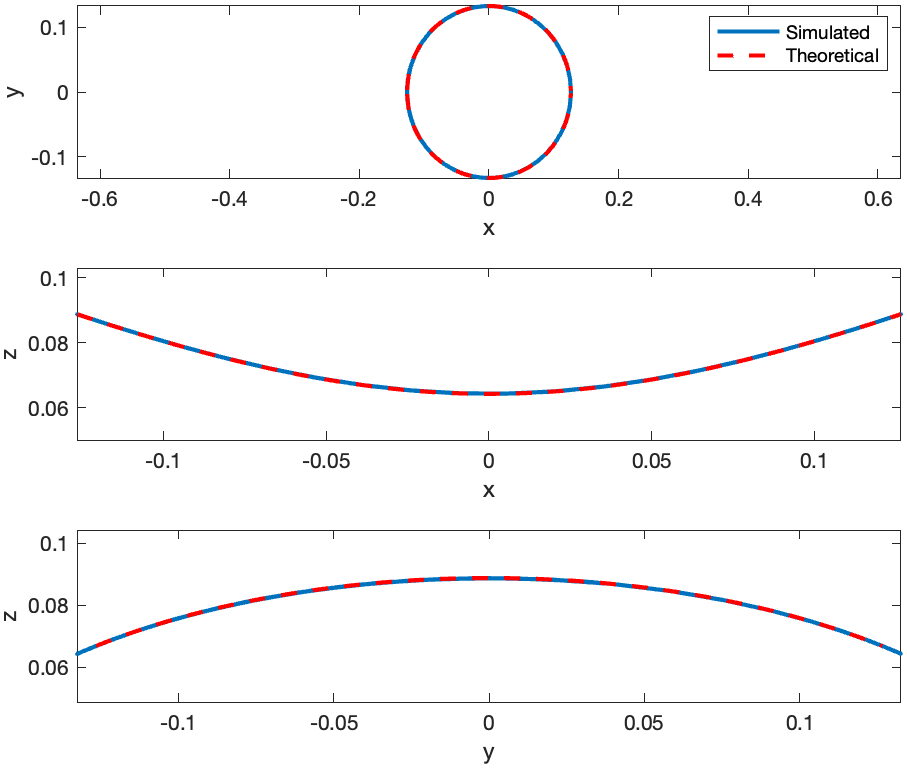
\includegraphics[width = 10cm]{Images/planar_polhode_random.png}
    \caption{Polhode Curve Projected onto Principally Aligned Cartesian Coordinate Planes}
    \label{fig:2d_polhode}
\end{figure}

\subsubsection{Repeat above steps changing initial conditions, e.g. setting angular velocity vector parallel to principal axis. Is the behavior according to expectations?} \label{sec:principally_aligned_omega}

Now with an initial condition of $\vec{\omega}_0 = \begin{bmatrix}
    10 & 0 & 0
\end{bmatrix}^T {}^{\circ}/s$ the magnitude of momentum and kinetic energy are 3056.1 kg m/s and 266.69 J respectively. With the angular velocity vector strictly aligned with one of the principal axes, the vector does not evolve in the principally oriented frame. That is, there is no gyroscopic coupling that causes the zero components of the angular velocity to increase or decrease. The vector components plotted over time are seen in Figure \ref{fig:sim_omegas_principal} 

\begin{figure}[H]
    \centering
    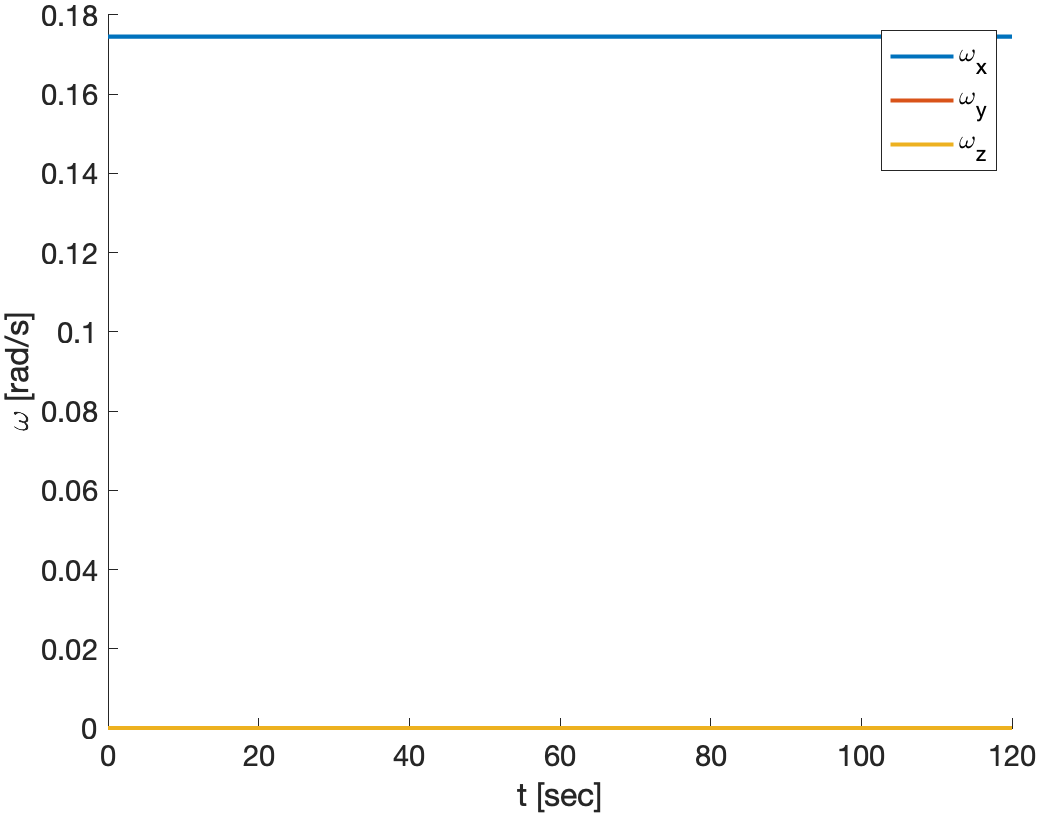
\includegraphics[width = 10cm]{Images/omega_prop_principal.png}
    \caption{Angular Velocity Vector Components for Principally Aligned Initical Conditions}
    \label{fig:sim_omegas_principal}
\end{figure}

The momentum and energy ellipsoids along with their semi-axis lengths can be seen plotted in Figures \ref{fig:momentum_axis_verification_princ} and \ref{fig:energy_axis_verification_princ} respectively.

\begin{figure}[H]
    \centering
    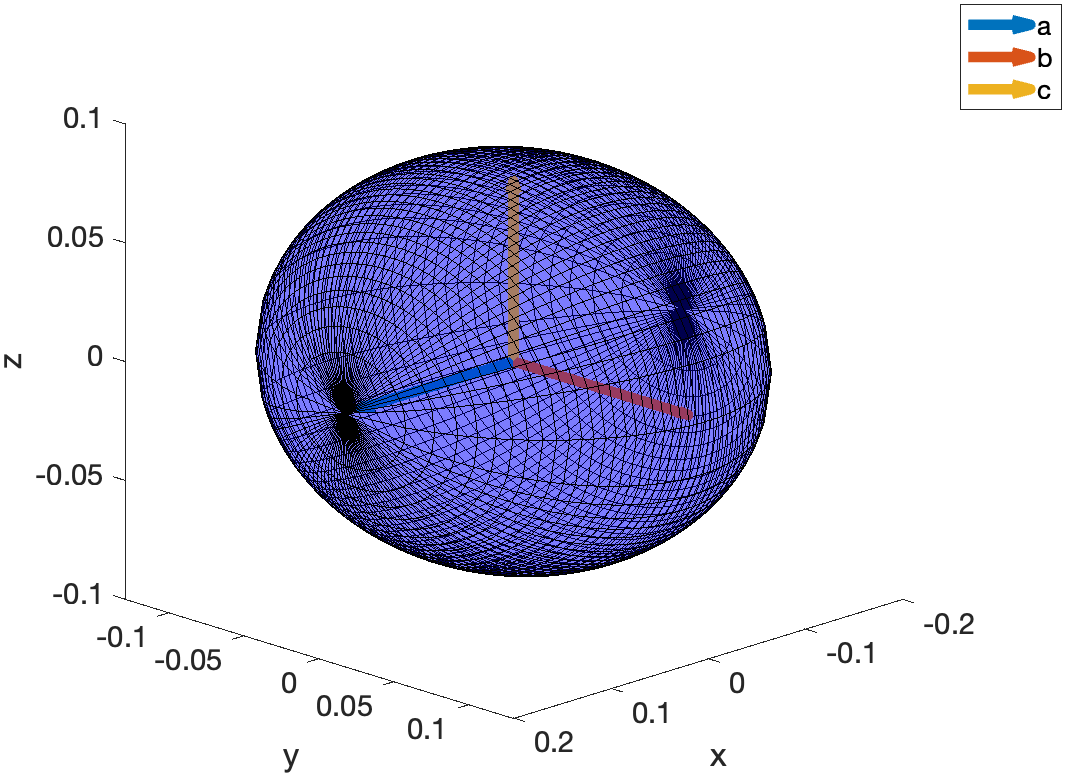
\includegraphics[width = 10cm]{Images/momentum_axes_principal.png}
    \caption{Momentum Ellipsoid and Semi-Axis Lengths for Principally Aligned Velocity Vector}
    \label{fig:momentum_axis_verification_princ}
\end{figure}

\begin{figure}[H]
    \centering
    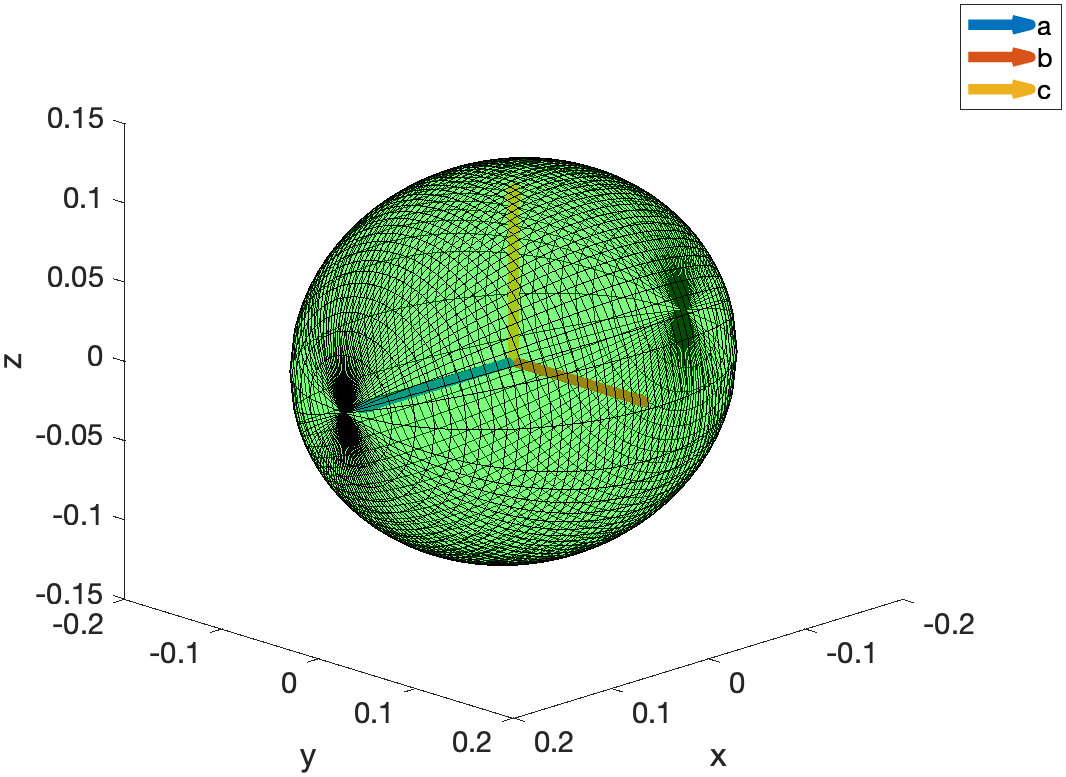
\includegraphics[width = 10cm]{Images/energy_axes_principal.png}
    \caption{Energy Ellipsoid and Semi-Axis Lengths for Principally Aligned Velocity Vector}
    \label{fig:energy_axis_verification_princ}
\end{figure}

This manifests in the polhode graph being a single point. Figure \ref{fig:ellipsoid_super_plot_principal} shows this point plotted at the intersection of the energy and momentum ellipsoids. The intersection in this case is strictly a point as the momentum ellipsoid is fully contained within the energy ellipsoid with two tangent points at  $10^{\circ}/s$ and $-10{}^{\circ}/s$ along the x-axis. 

\begin{figure}[H]
    \centering
    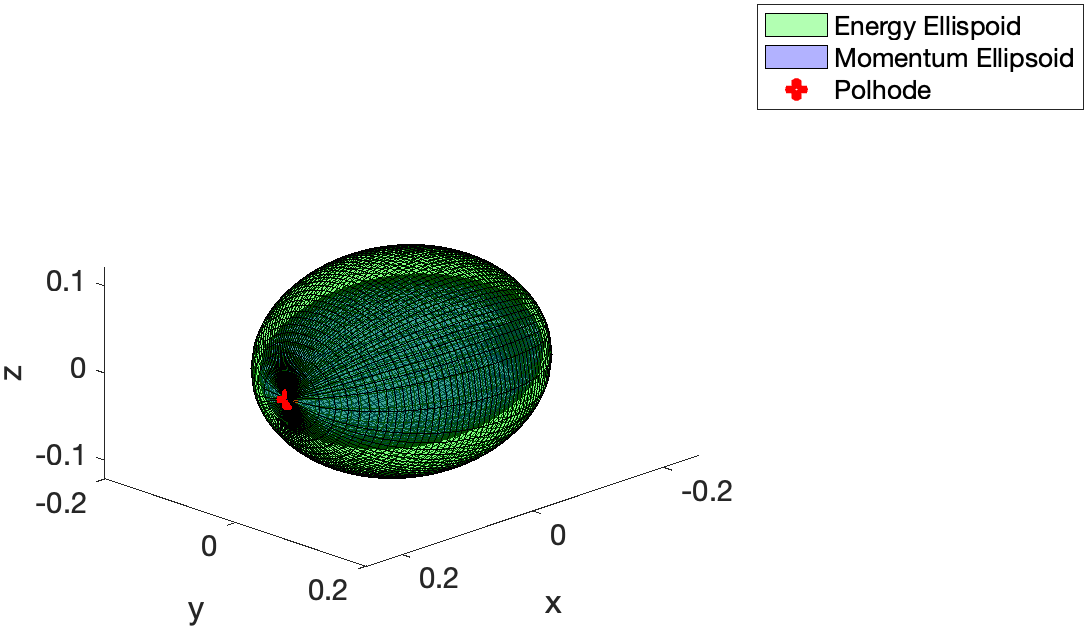
\includegraphics[width = 12cm] {Images/ellipsoid_polhode_principal.png}
    \caption{Momentum and Energy Ellipsoids and Polhode for Angular Velocity Aligned with a Principal Axis}
    \label{fig:ellipsoid_super_plot_principal}
\end{figure}

The polhode projected onto 2D axes is a single point that should lie along the theoretical curve described in Equations \ref{eq:polhode1}, \ref{eq:polhode2}, and \ref{eq:polhode3}. This is shown to hold true in Figure \ref{fig:2d_polhode_principal}. The points from simulation are seen to coincide with the theoretical expectation within an error on the order of magnitude of $10^{-8}$. Additionally, with these initial conditions, the quantity $L^2/2T$ evaluates to 17510 kg m\textsuperscript{2} which lies within the specified bounds described in \ref{sec:principal_inertia_def_and_calc}..

\begin{figure}[H]
    \centering
    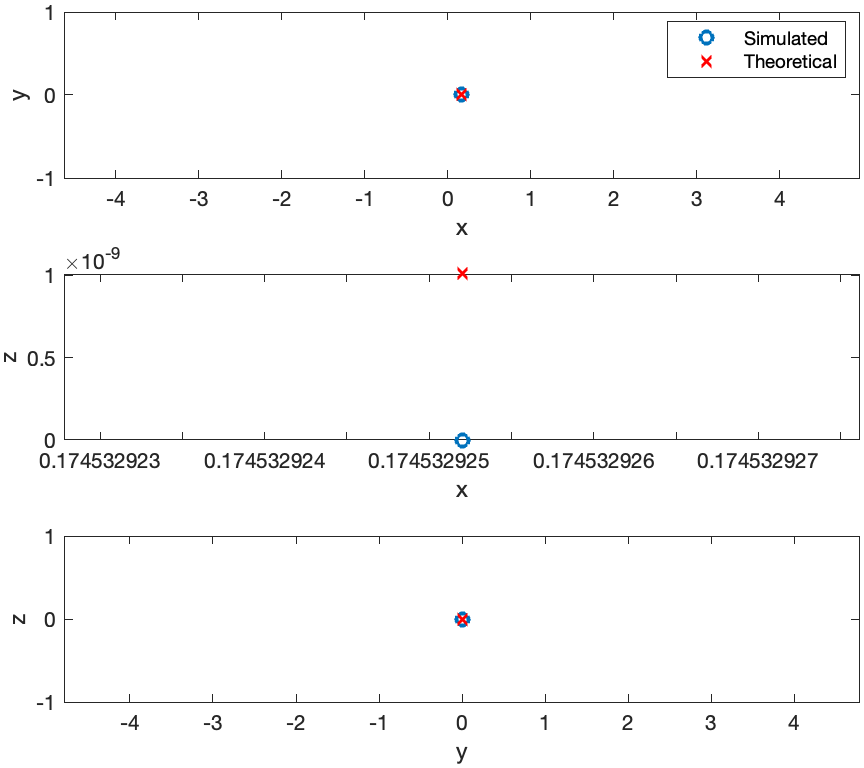
\includegraphics[width = 10cm]{Images/planar_polhode_principal.png}
    \caption{Projected Polhode Curve for Principally Aligned Angular Velocity Vector}
    \label{fig:2d_polhode_principal}
\end{figure}

The code used to perform all calculations and plots for Sections \ref{sec:principal_inertia_def_and_calc} -- \ref{sec:principally_aligned_omega} is listed below.

\lstinputlisting{Code/HW2main.m}
\section{\Large PROBLEM SET 3}
\subsection{Problem 3}

\subsubsection{Impose that satellite is axial-symmetric (i.e., impose $I_x=I_y\neq I_z$). Repeat numerical simulation from previous pset using initial condition 4) from previous pset.}

The principal inertia of the Aqua satellite is listed in \ref{sec:principal_inertia_def_and_calc}. Imposing that $I_y=I_x$, the axis-symmetric representation of the satellite is seen below.



\subsubsection{Program analytical solution for axial-symmetric satellite. Compute it at same time steps and from same initial conditions.}

\subsubsection{Compare numerical and analytical solutions. Plot differences (errors), do not only superimpose absolute values. Tune numerical integrator for large discrepancies. Are angular velocity vector and angular momentum vector changing according to theory in principal axes?}

\subsubsection{Program Kinematic equations of motion correspondent to a nominal attitude parameterization of your choice.}

\subsubsection{Program Kinematic equations of motion correspondent to a different attitude parameterization from the previous step. This is used for comparison, to get familiar with different approaches, and as fall back solution in the case of singularities.}

\subsubsection{Go back to your original satellite inertia tensor. Numerically integrate Euler AND Kinematic equations from arbitrary initial conditions (warning: stay far from singularity of adopted parameterization). Multiple revolutions. The output is the evolution of the attitude parameters over time. These attitude parameters describe orientation of principal axes relative to inertial axes.}

\subsubsection{Since inertial position, velocity, and attitude, are known at the same time throughout the simulation, it is now possible to express vectors in the reference systems of interest}

%%%%%%%%%%%%%%%%%%%%%%%%%%%%%%%%%%%%%%%%%%%%%%%%%%%%%%%%%%%%%%%%%%%%%%%%%%%%%%%%%%%%%%%%%%%%%%%%%%%%%%%%%%%%%%%%%%%%%%%%%%%%%%%%%%%%%%%%%%%%%%%%%%%%%%%%%%%%%%%%%%%%%%%%%%%%%%%%%%%%%%%%%%%%%%%%%%%%%%%%%%%%%%%%%%%%%%%%%%% 
\section{\Large CONCLUSION}

\bibliographystyle{IEEEtran}
\bibliography{refs}


\end{document}